\documentclass[11pt,a4paper]{article}
\usepackage[margin=0.9in]{geometry}
\usepackage{graphicx}
\usepackage{booktabs}
\usepackage{longtable}
\usepackage{array}
\usepackage{float}
\usepackage{hyperref}
\usepackage{amsmath}
\usepackage{amssymb}
\usepackage{xcolor}
\hypersetup{colorlinks=true, linkcolor=blue, urlcolor=blue}
\setlength{\parskip}{0.45em}
\setlength{\parindent}{0pt}
\graphicspath{{260403_report_assets/}}

\begin{document}

\begin{titlepage}
\centering
{\LARGE 260403\_report\par}
\vspace{0.8cm}
{\Large Comprehensive Technical Report for the SpeedEstimation Project\par}
\vspace{0.8cm}
{\large Repository: \texttt{/home/chanyoungko/IIT/SpeedEstimation}\par}
\vspace{0.4cm}
{\large Date: 2026-04-03\par}
\vspace{1.2cm}
\begin{minipage}{0.92\linewidth}
\small
This report consolidates the full project history of the SpeedEstimation repository, including data protocol decisions, feature generation, preprocessing, model architectures, training methodology, archive-by-archive experiments, quantitative results, qualitative plots, compute/deployment implications, and the corrected season3 relaunch after the ground-truth target definition was revised from treadmill belt speed to \texttt{common/v\_Y\_true}.
\end{minipage}
\vfill
\begin{minipage}{0.92\linewidth}
\small
Intended audience: repository maintainers, collaborators, and any reader who needs to understand what was tried, what worked, what failed, what changed over time, and which models are the most credible baselines under the old and corrected target protocols.
\end{minipage}
\end{titlepage}

\tableofcontents
\clearpage

\section{Executive Summary}

The SpeedEstimation project studies treadmill walking speed estimation from synchronized biomechanics signals: motion capture joint kinematics, trunk IMU, force plates, exoskeleton torques, and subject anthropometrics. The repository evolved through many archives in season1 and season2, and then required a season3 restart when it was discovered that the training target used in seasons1--2 was \texttt{treadmill/left/speed\_leftbelt} instead of the intended \texttt{common/v\_Y\_true}.

The most important high-level conclusions are:

\begin{itemize}
\item Under the original season1/season2 target protocol, the strongest family was the body-frame IMU plus IMU-integrated-speed baseline. The canonical representative is \texttt{exp\_A5\_bodyframe\_plus\_imuint}, which reached MAE \(\approx 0.01125\).
\item A large number of later ideas were tested: residual skip models, delta targets, soft prior losses, observer-style models, confidence-weighted fusion, distillation, sensor-light models, and tiny deployment-oriented models.
\item Most new methods did not beat the strongest season2 baseline in absolute MAE, but several created useful \emph{non-accuracy} contributions: smaller models, lower sensor dependence, and more deployment-friendly structures.
\item After correcting the target protocol in season3, the ranking changed. The best season3 models were \texttt{raw\_full} and \texttt{imuint\_full} families, not the season2 body-frame fusion family. The season3 best model was \texttt{exp\_S3A1\_G009\_raw\_full\_w200\_base\_pglpf} with MAE \(\approx 0.02439\).
\item The corrected season3 results imply that season1 and season2 remain useful as method-development history, but they should not be mixed numerically with season3 without explicitly stating the target mismatch.
\item Real-time deployment remained a hard requirement throughout the project. Models were therefore kept causal, single-pass, and reasonably small, and several archives explicitly explored parameter-count and sensor-count reductions.
\end{itemize}

\section{Project Scope and Hard Constraints}

The repository estimates walking speed in a treadmill + exoskeleton setting. The end goal is not just offline accuracy. The final model must remain feasible for online use, which means that the entire inference path must be lightweight:

\begin{itemize}
\item feature extraction must be causal or at least online-computable,
\item derived signals must not depend on non-causal future information during deployment,
\item the neural model must remain small enough for real-time use,
\item the evaluation story must distinguish between causal inference and non-causal visualization or analysis.
\end{itemize}

This constraint shaped nearly every design decision. For example:

\begin{itemize}
\item \texttt{derived/imu\_integrated\_speed} uses a causal leaky integrator and causal low-pass filter,
\item \texttt{derived/model\_com\_speed} uses causal filtering,
\item TCN-based and GRU-based causal models were preferred over heavier sequence models,
\item test-time augmentation, feature importance, and detailed plotting were treated as analysis tools, not deployable inference paths.
\end{itemize}

\section{Repository Structure}

The repository is organized around four main layers:

\begin{itemize}
\item \texttt{data/}: H5 loading, preprocessing, trial caching, body-frame IMU conversion, model-based COM speed, and IMU-integrated speed.
\item \texttt{core/}: model definitions, sliding-window dataset construction, target transforms, and auxiliary losses.
\item \texttt{training/}: end-to-end training loop, scaling, checkpointing, metrics, and distillation support.
\item top-level scripts: \texttt{SpeedEstimator\_TCN\_MLP\_experiments.py}, \texttt{compare\_results.py}, \texttt{train.sh}, \texttt{eval\_server.sh}, and \texttt{cpu\_eval.sh}.
\end{itemize}

Key implementation files:

\begin{itemize}
\item \texttt{data/loader.py}: loads trial data, computes derived features on the fly, handles input LPF, output LPF, and the trial-level cache.
\item \texttt{data/body\_frame.py}: computes body-aligned IMU features from quaternion-calibrated trunk IMU signals.
\item \texttt{data/model\_com\_speed.py}: implements model-based COM speed and IMU-integrated speed priors.
\item \texttt{core/models.py}: defines the TCN/GRU family, attention, multiscale, observer, and fusion models.
\item \texttt{core/datasets.py}: defines sliding-window sampling, time-warp augmentation, and target transforms.
\item \texttt{core/losses.py}: defines smoothness, gradient-penalty, and prior-alignment losses.
\item \texttt{training/trainer.py}: orchestrates model fitting, validation, testing, logging, distillation, and metrics export.
\item \texttt{compare\_results.py}: performs analysis, plotting, ablations, permutation importance, and archive-level summaries.
\end{itemize}

\section{Dataset, Trial Structure, and Ground-Truth Protocols}

\subsection{Dataset organization}

The repository uses \texttt{combined\_data.h5} and earlier related H5 files. The data hierarchy is:

\[
\texttt{Subject / Condition / Level / Trial}
\]

Milestone2 experiments use subjects \texttt{m2\_S001} through \texttt{m2\_S008}. Common conditions include:

\begin{itemize}
\item \texttt{level\_075mps}
\item \texttt{level\_100mps}
\item \texttt{level\_125mps}
\item \texttt{accel\_sine}
\item \texttt{decline\_5deg}
\item \texttt{incline\_10deg}
\item \texttt{stopandgo}
\end{itemize}

The sampling rate is 100\,Hz.

\subsection{Protocol split: old target vs corrected target}

One of the most important findings late in the project was that seasons1--2 had been trained against the wrong ground-truth target. There are therefore two distinct experimental protocols in this repository:

\begin{enumerate}
\item \textbf{Old protocol (season1 and season2):}
  \begin{itemize}
  \item output variable: \texttt{treadmill/left/speed\_leftbelt}
  \item preprocessing: bidirectional Butterworth low-pass filter via \texttt{scipy.signal.filtfilt}
  \item typical cutoff: 0.5\,Hz, order 4
  \end{itemize}
\item \textbf{Corrected protocol (season3 onward):}
  \begin{itemize}
  \item output variable: \texttt{common/v\_Y\_true}
  \item preprocessing: the same bidirectional low-pass filter, again typically 0.5\,Hz, order 4
  \end{itemize}
\end{enumerate}

This distinction matters. Season1/2 numbers are still historically useful for understanding which design ideas worked under the old protocol, but they are not numerically interchangeable with season3.

\begin{figure}[H]
\centering
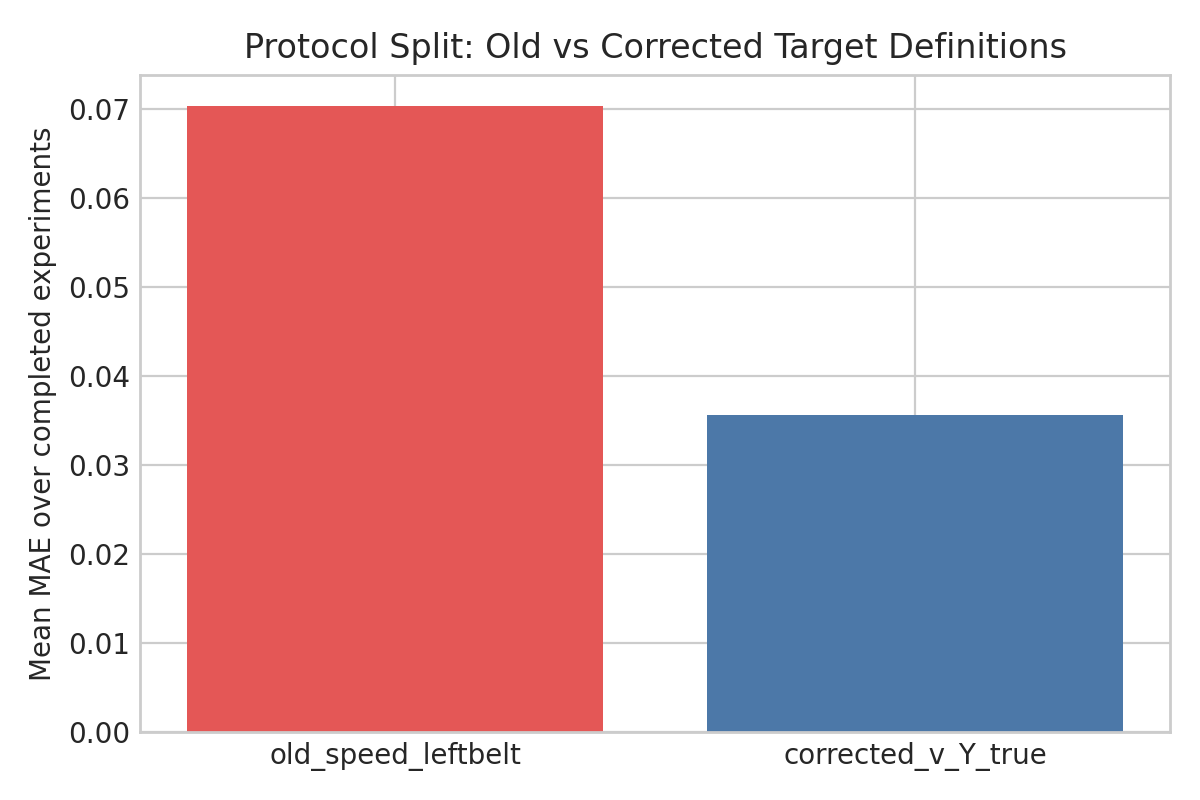
\includegraphics[width=0.68\linewidth]{target_protocol_split.png}
\caption{Mean MAE over completed experiments under the old protocol (\texttt{speed\_leftbelt}) and the corrected protocol (\texttt{v\_Y\_true}). This figure should \emph{not} be interpreted as a direct method comparison across seasons; it simply visualizes that the protocol split is real and significant.}
\end{figure}

\subsection{Target filtering implementation}

Output targets are filtered in \texttt{data/utils.py} through:

\[
\texttt{butter\_lowpass\_filter}(x, f_c, f_s, \text{order})
\]

which uses \texttt{filtfilt}. This means the target smoothing is zero-phase and bidirectional. That is appropriate for offline training targets, but not itself a deployable causal target-generation procedure.

\section{Input Features and How They Are Generated}

\subsection{Overview of feature groups}

Across the full project, the main input groups were:

\begin{itemize}
\item \textbf{Motion capture joint kinematics} (\texttt{mocap/kin\_q}):
  hip flexion, knee angle, and ankle angle for left/right, plus first and second derivatives.
\item \textbf{Raw trunk IMU} (\texttt{robot/back\_imu}):
  roll, pitch, yaw, and a legacy forward velocity estimate in some season1/season3 raw-family experiments.
\item \textbf{Body-frame trunk IMU} (\texttt{derived/body\_frame\_imu}):
  body-aligned accelerations and gyroscope signals plus overground-like forward acceleration.
\item \textbf{IMU-integrated speed prior} (\texttt{derived/imu\_integrated\_speed}).
\item \textbf{Model-based COM speed prior} (\texttt{derived/model\_com\_speed}).
\item \textbf{Exoskeleton torque} (\texttt{robot/left}, \texttt{robot/right}).
\item \textbf{Force plate signals} (\texttt{forceplate/grf/left}, \texttt{forceplate/grf/right}) including contact bits.
\item \textbf{Subject information} (\texttt{sub\_info}) limited to height and weight.
\end{itemize}

\textbf{Important exclusion:} \texttt{common/assist\_level} was explicitly checked and was \emph{not} used in the trained models summarized here. The repository rule now forbids adding it to future experiments.

\subsection{Kinematic feature generation}

Joint-angle inputs were usually defined as:

\begin{itemize}
\item six raw angles:
  \texttt{hip\_flexion\_l/r}, \texttt{knee\_angle\_l/r}, \texttt{ankle\_angle\_l/r}
\item six angular velocities:
  the corresponding \texttt{\_dot} channels
\item six angular accelerations:
  the corresponding \texttt{\_ddot} channels
\end{itemize}

The derivatives are generated on the fly in \texttt{data/loader.py} using:

\[
\dot{q}(t) \approx \nabla q(t)\cdot f_s,\qquad
\ddot{q}(t) \approx \nabla \dot{q}(t)\cdot f_s
\]

and then low-pass filtered. In the default path, derived velocities/accelerations were filtered at 30\,Hz unless a per-group LPF override was provided.

\subsection{Raw IMU feature path}

The raw IMU path used \texttt{robot/back\_imu} features such as roll, pitch, yaw, and the legacy \texttt{vel\_forward}. This was the original season1-style representation and remained important again in season3 after the target was corrected.

\subsection{Body-frame IMU feature path}

The body-frame IMU path is defined in \texttt{data/body\_frame.py}. It transforms raw trunk IMU signals into a body-aligned frame with axes:

\[
X=\text{right},\quad Y=\text{forward},\quad Z=\text{up}
\]

The processing pipeline is:

\begin{enumerate}
\item quaternion sign canonicalization to maintain temporal continuity,
\item local-to-global-like rotation using the IMU quaternion,
\item standing-based estimate of the upward axis from gravity,
\item causal forward-axis estimation via sliding-window PCA on horizontal acceleration,
\item orthonormal body-frame reconstruction,
\item gravity removal,
\item projection of acceleration and angular velocity into the body frame,
\item addition of treadmill acceleration to form an overground-like forward-acceleration channel.
\end{enumerate}

The main derived channels are:

\begin{itemize}
\item \texttt{accel\_right}
\item \texttt{accel\_forward}
\item \texttt{accel\_up}
\item \texttt{gyro\_right}
\item \texttt{gyro\_forward}
\item \texttt{gyro\_up}
\item \texttt{forward\_accel\_overground}
\end{itemize}

The last one is particularly important:

\[
a_{\text{forward,overground}} = a_{\text{body},Y} + a_{\text{treadmill}}
\]

This feature was one of the central ideas of season2 and remained part of the strongest physics-guided input sets.

\subsection{IMU-integrated speed}

The IMU-integrated speed prior is implemented in \texttt{data/model\_com\_speed.py}. It is not a naive integration of raw accelerometer data. The actual recipe is:

\begin{enumerate}
\item compute body-frame forward acceleration,
\item add treadmill acceleration to obtain overground-equivalent forward acceleration,
\item run a leaky integrator,
\item apply a causal low-pass filter.
\end{enumerate}

The recurrence is:

\[
v_t = \alpha v_{t-1} + a_t \Delta t
\]

followed by causal LPF smoothing. Under the old target protocol, this was consistently the strongest single physics-inspired prior.

\subsection{Model-based COM speed}

The model-based COM speed prior approximates pelvis-center forward speed relative to the stance foot using joint kinematics and stance detection:

\begin{itemize}
\item hip and knee angles define segment orientation,
\item pelvis pitch and yaw contribute to pelvis-center motion,
\item GRF stance detection chooses the left, right, or averaged stance-leg chain,
\item segment lengths are estimated from anthropometric ratios of height.
\end{itemize}

This feature was attractive from a biomechanics standpoint, but it rarely beat the IMU-integrated-speed family in actual experiments.

\subsection{Force plates, contact, torque, and subject information}

GRF signals contributed \((x,y,z)\) channels for each side plus derived binary contact. Torque channels came from \texttt{robot/left/torque} and \texttt{robot/right/torque}. Subject information was limited to height and weight and was broadcast along the trial time axis.

\subsection{Input filtering variants}

Several archives explored input filtering:

\begin{itemize}
\item global input LPF
\item per-group LPF, such as:
  \begin{itemize}
  \item accelerations and IMU at 8\,Hz,
  \item GRF at 12\,Hz
  \end{itemize}
\end{itemize}

In season3, the design sweep encoded these as \texttt{none}, \texttt{glpf8}, and \texttt{pglpf}. The mean-MAE comparison is shown below.

\begin{figure}[H]
\centering
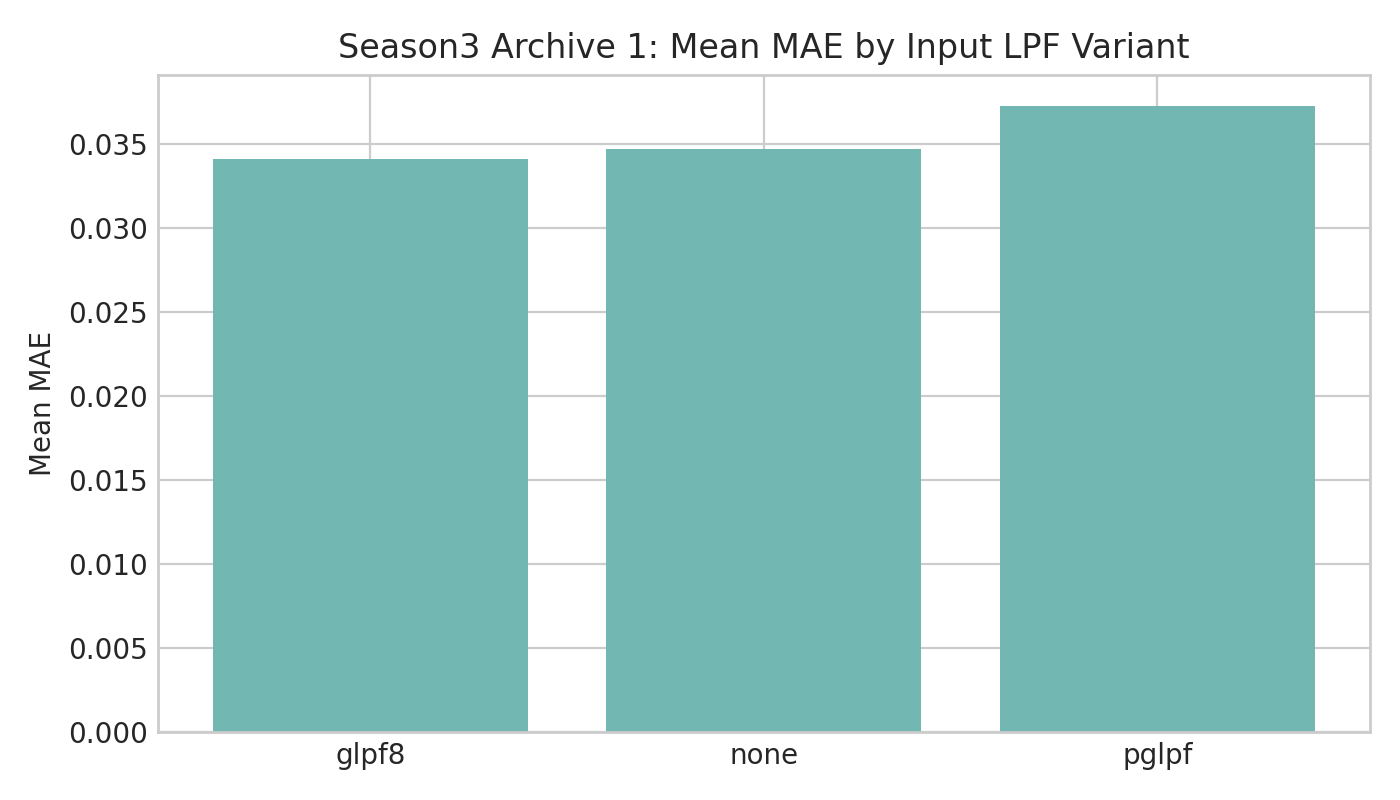
\includegraphics[width=0.62\linewidth]{season3_input_lpf_mean_mae.png}
\caption{Season3 archive\_1 mean MAE by input LPF variant. On average, \texttt{glpf8} was best, but the single best model still came from the \texttt{pglpf} branch.}
\end{figure}

\section{Sliding Windows, Normalization, Augmentation, and Target Transforms}

\subsection{Windowing}

The standard formulation uses sliding windows:

\begin{itemize}
\item training stride typically 5,
\item inference stride 1 for full evaluation and 3 for fast evaluation,
\item output delay \(y\_\text{delay}=5\), i.e.\ about 50\,ms at 100\,Hz,
\item horizon commonly represented as \texttt{est\_tick\_ranges: [5]}.
\end{itemize}

Representative window sizes:

\begin{itemize}
\item 300 samples: accuracy-oriented baseline
\item 200 samples: strongest season3 average
\item 150 samples: lighter deployment-oriented setting
\item 120 samples: tiny-model exploration
\end{itemize}

\begin{figure}[H]
\centering
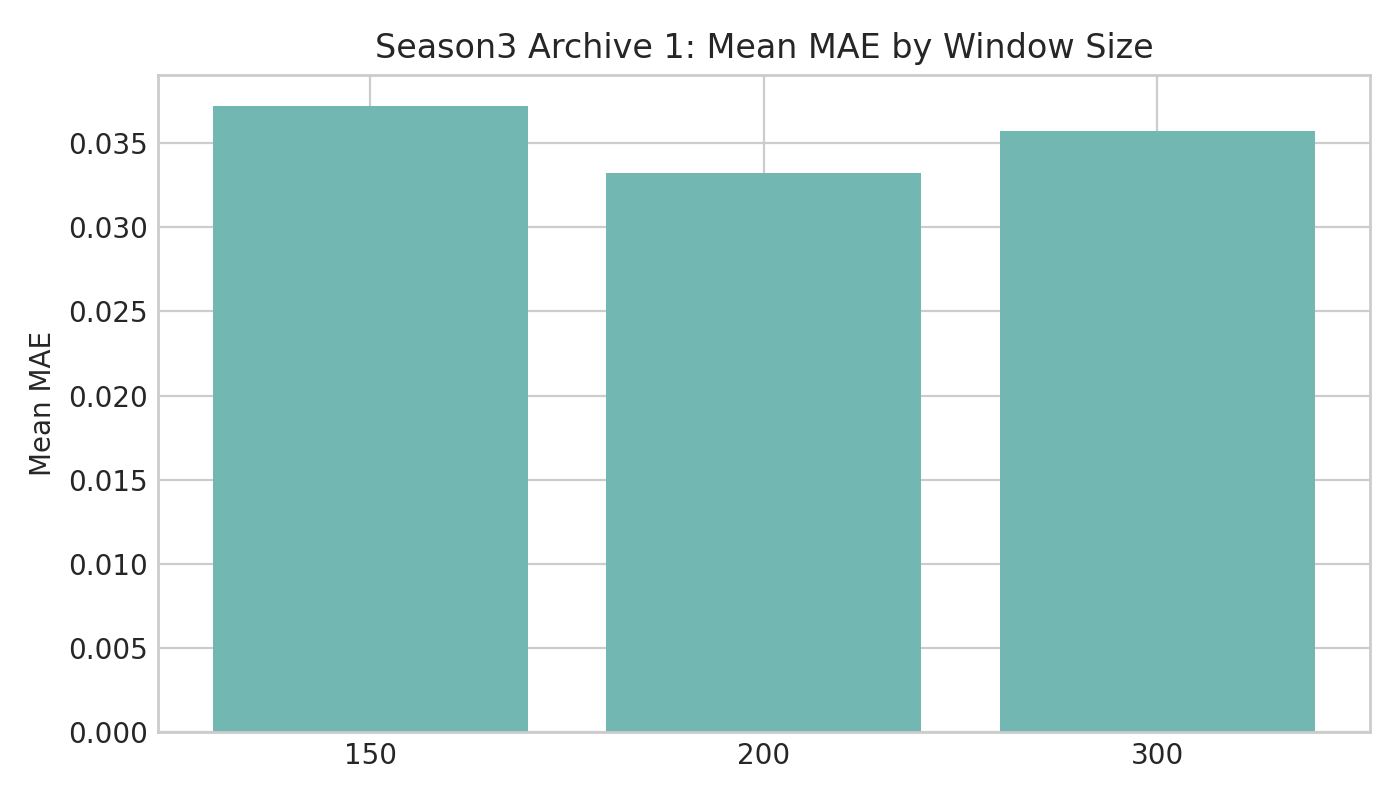
\includegraphics[width=0.62\linewidth]{season3_window_mean_mae.png}
\caption{Season3 archive\_1 mean MAE by window size. Window 200 was the strongest average setting.}
\end{figure}

\subsection{Normalization}

The standard setting uses standard normalization. Many models also enable instance normalization at the input stage. This became the dominant choice in later archives.

\subsection{Augmentation}

The dataset and trainer support:

\begin{itemize}
\item additive Gaussian noise,
\item optional per-dimension noise,
\item random time warping (\texttt{core/datasets.py}),
\item archive-specific robustness sweeps such as season2 noise and LPF experiments.
\end{itemize}

\subsection{Target transforms}

Later archives introduced a target-transform mechanism, mainly for delta-target experiments. The dataset module supports:

\[
y' = y - \text{base}(x)
\]

with the inverse applied during evaluation to restore absolute-speed metrics. This was used heavily in archive\_4.

\section{Model Families}

\subsection{Baseline family: TCN + GRU head}

The canonical strong baseline is \texttt{TCN\_GRU}. It uses:

\begin{itemize}
\item a causal TCN encoder with residual temporal blocks,
\item increasing dilation across layers,
\item a GRU head on the encoder sequence,
\item a final linear projection to the target horizon.
\end{itemize}

The most common channel setting was:

\[
[32, 32, 64, 64, 128, 128]
\]

with kernel size 5 and GRU hidden size 32.

\subsection{TCN\_MLP and early variants}

\texttt{TCN\_MLP} uses the same TCN encoder but replaces the GRU head with an MLP head. It remained a useful baseline but the TCN+GRU family dominated most later comparisons.

\subsection{Stance-gated and attention variants}

\texttt{StanceGatedTCN} applies a learned multiplicative gate to the input sequence before encoding. \texttt{AttentionTCN} uses temporal attention pooling over the encoded sequence instead of just taking the last step. These were explored as potentially more adaptive sequence summaries but did not become dominant.

\subsection{Multiscale and causal-smoothing variants}

\texttt{MultiScaleTCN\_GRU} uses parallel TCN branches with different kernel sizes and then fuses them before the GRU. \texttt{CausalSmoothTCN\_GRU} adds a learnable depthwise causal smoothing layer after the GRU. Both were motivated by the idea that speed dynamics might require both fast and slow context, but empirical gains were limited.

\subsection{Observer-style model}

\texttt{ObserverTCN\_GRU} introduced a propagated prior and a learned correction:

\[
\hat{y} = \text{propagated prior} + \sigma(g)\cdot \Delta
\]

with optional acceleration-driven propagation. This was one of the more ambitious ideas in archive\_5 but did not work reliably.

\subsection{Fusion model}

\texttt{FusionTCN\_GRU} was the most useful later model family. It performs confidence-weighted fusion between:

\begin{itemize}
\item one learned branch,
\item one or more prior channels taken directly from the input at the latest time step.
\end{itemize}

If the sources are \(s_1,\ldots,s_K\) and the network predicts logits \(z_1,\ldots,z_K\), then:

\[
w_k = \text{softmax}(z_k / \tau), \qquad
\hat{y} = \sum_{k=1}^{K} w_k s_k
\]

This family never overtook the strongest old-protocol baseline in absolute MAE, but it produced the clearest deployment-oriented tradeoffs.

\subsection{Residual skip connection}

Residual skip support was added at the model level:

\[
\hat{y} = f(x) + x_{t,\text{idx}}
\]

where the base channel is read from the latest input timestep before normalization. This mechanism powered many archive\_3 experiments and mostly failed in practice.

\section{Training Infrastructure and Losses}

\subsection{Core training recipe}

Typical settings across successful archives:

\begin{itemize}
\item optimizer: AdamW
\item loss: Huber with \(\delta = 0.1\)
\item epochs: 30
\item learning rate: 0.001
\item weight decay: 0.001
\item mixed precision: enabled
\item early stopping patience: 10
\item cosine schedule with \(T_0=10\)
\item batch size: 128, validation batch size: 256
\end{itemize}

\subsection{Custom losses}

\texttt{core/losses.py} supports:

\begin{itemize}
\item smoothness loss,
\item gradient-penalty loss limiting excessive speed jumps,
\item frequency-penalty loss,
\item prior-alignment loss, which softly encourages predictions toward a specified prior channel.
\end{itemize}

The prior-alignment loss was the most useful of these additions and was especially relevant in archive\_4 and archive\_6.

\subsection{Distillation}

Distillation support was added in \texttt{training/trainer.py}. A teacher model can be loaded from a previous experiment folder, normalized into the teacher's input space, and used to add a student-teacher MSE term. This was explored in archive\_5. It was implemented correctly, but it did not generate a convincing empirical gain.

\section{Evaluation and Analysis Infrastructure}

\subsection{LOSO setting}

Most season2 and season3 experiments summarized here use a single-LOSO held-out subject, usually \texttt{m2\_S008}. This is sufficient for controlled archive comparisons, but not equivalent to a full all-subject LOSO publication result.

\subsection{compare\_results pipeline}

\texttt{compare\_results.py} performs:

\begin{itemize}
\item full-sequence evaluation,
\item lag and smoothness metrics,
\item qualitative per-condition trajectory plots,
\item archive-level ablation reports,
\item optional permutation feature importance.
\end{itemize}

During the season3 plot generation work, several bugs and bottlenecks were fixed:

\begin{itemize}
\item \texttt{target\_dir} selection was corrected so config-specific analysis would not silently scan unrelated experiment folders,
\item \texttt{eval\_stride} propagation was fixed for single-experiment detailed analysis,
\item memory usage was reduced by removing unnecessary full concatenation of raw input batches,
\item the single-model detailed path was fixed to reconstruct the output dimension correctly.
\end{itemize}

One known remaining issue is that the feature-importance tail of the evaluation path still calls an undefined name-generation helper in some cases. This does not invalidate the already generated plots, but it means feature-importance outputs were not consistently available for every later archive.

\section{Archive-by-Archive History}

\subsection{Season1 baseline and rounds}

Season1 started from raw kinematics plus raw trunk IMU representations and explored:

\begin{itemize}
\item global-acceleration style preprocessing,
\item smoothness losses,
\item input filtering,
\item time-warp augmentation,
\item noise augmentation and TTA.
\end{itemize}

Important season1 checkpoints:

\begin{itemize}
\item baseline: MAE \(\approx 0.01054\)
\item archive\_round3 best: \texttt{exp\_F1\_global\_acc\_additive}, MAE \(\approx 0.01067\)
\item archive\_round8 best: \texttt{exp\_C2\_noise\_010}, MAE \(\approx 0.01395\)
\end{itemize}

At the time, this looked like a mature baseline. Later, however, it became clear that all of these experiments were trained against the old target protocol.

\subsection{Season2 archive\_1: body-frame representation and speed priors}

archive\_1 was the first major representation shift. The main question was whether the trunk IMU should be expressed in a body-aligned frame, and whether physics-guided speed priors should be fused into the input.

Representative result:

\begin{itemize}
\item \texttt{exp\_S2\_imu\_speed\_only}: MAE \(\approx 0.01125\)
\end{itemize}

Main conclusion:

\begin{itemize}
\item IMU-integrated speed was a genuinely useful prior,
\item body-frame representation was helpful in the context of that prior,
\item model-based COM speed was weaker than expected.
\end{itemize}

\subsection{Season2 archive\_2: main ablation archive}

archive\_2 is the most important old-protocol ablation archive. It compared raw IMU, body-frame IMU, old forward-velocity signals, IMU-integrated speed, dual-prior combinations, robustness tweaks, and structure changes.

The key winner was:

\begin{itemize}
\item \texttt{exp\_A5\_bodyframe\_plus\_imuint}, MAE \(\approx 0.01125\)
\end{itemize}

This result became the de facto strong baseline for the remainder of season2.

\subsection{Season2 archive\_3: hard residual skip}

archive\_3 tested the idea that the network should only predict a correction on top of a physics prior. This was an intuitively attractive, paper-like idea, but it failed in practice. Many residual formulations diverged badly or landed far above the strong baseline.

The archive best was still poor:

\begin{itemize}
\item \texttt{exp\_A4\_dualphysics\_modelcom\_residual}, MAE \(\approx 0.10665\)
\end{itemize}

This archive is best understood as a negative-result archive.

\subsection{Season2 archive\_4: delta targets and soft priors}

archive\_4 softened the residual idea. Instead of hard skip addition, it introduced:

\begin{itemize}
\item delta-target training,
\item soft prior-alignment loss.
\end{itemize}

This stabilized training considerably relative to archive\_3, but it still did not beat the archive\_2 baseline. The best run in archive\_4 was simply a reproduction of the old best baseline.

\subsection{Season2 archive\_5: observer, fusion, distillation}

archive\_5 explored three more ambitious directions:

\begin{itemize}
\item observer-style propagated prior + learned correction,
\item confidence-weighted fusion between priors and learned estimate,
\item teacher-student distillation.
\end{itemize}

Outcome:

\begin{itemize}
\item observer models mostly failed,
\item distillation did not help,
\item fusion was the only clearly positive new direction.
\end{itemize}

Representative fusion result:

\begin{itemize}
\item \texttt{exp\_S2A5\_B1\_fusion\_imuint}, MAE \(\approx 0.01474\)
\end{itemize}

\subsection{Season2 archive\_6: deployability and sensor-light models}

archive\_6 was the final season2 push toward practical contribution beyond raw MAE. It focused on:

\begin{itemize}
\item dual-prior fusion with soft prior alignment,
\item real-time lightweight variants,
\item no-GRF / no-torque sensor-light variants,
\item tiny Pareto points.
\end{itemize}

Key takeaways:

\begin{itemize}
\item the strongest fusion variant was \texttt{exp\_S2A6\_A4\_fusion\_dual\_softprior}, MAE \(\approx 0.01860\),
\item a very practical sensor-light model was \texttt{exp\_S2A6\_C2\_fusion\_imuint\_nogrf\_notorque}, MAE \(\approx 0.02454\),
\item a tiny Pareto point was \texttt{exp\_S2A6\_B3\_fusion\_dual\_tiny120}, MAE \(\approx 0.04028\) with only about 74k parameters.
\end{itemize}

\subsection{Season3 archive\_1: corrected-target relaunch}

Once the target issue was identified, the project was restarted in season3. Instead of re-running only a few experiments, archive\_1 was expanded to 186 configs so that the corrected protocol could be screened systematically.

The sweep factors included:

\begin{itemize}
\item family: raw\_full, raw\_lite, bf\_full, bf\_lite, imuint\_full, imuint\_lite, fusionimu\_full, fusionimu\_lite, dual\_full, dualsoft\_full
\item window size: 300, 200, 150
\item model size: base, compact
\item input LPF variant: none, glpf8, pglpf
\end{itemize}

All 186 configs completed successfully.

\section{Quantitative Summary}

\subsection{Best experiment per archive}

Table~\ref{tab:archive-best} summarizes the best completed result from each archive or season bucket available in the repository.

\begin{table}[H]
\centering
\small
\caption{Best experiment from each archive among completed runs in the repository.}
\label{tab:archive-best}
\resizebox{\linewidth}{!}{%
\begin{tabular}{p{3.0cm}p{7.6cm}rrrr}
\toprule
Archive & Best experiment & MAE & RMSE & Params & Latency (ms) \\
\midrule
archive\_season1/archive\_round1 & exp\_multistep\_H10 & 0.01269 & 0.02782 & 401766 & 2.618 \\
archive\_season1/archive\_round3 & exp\_F1\_global\_acc\_additive & 0.01067 & 0.02859 & 409287 & 2.4276 \\
archive\_season1/archive\_round4 & exp\_A1\_smooth\_loss\_light & 0.01118 & 0.02792 & 409157 & 2.5291 \\
archive\_season1/archive\_round5 & exp\_D4\_input\_lpf\_deep & 0.01229 & 0.03098 & 738241 & 3.1103 \\
archive\_season1/archive\_round6 & exp\_E2\_augment\_time\_warp & 0.01135 & 0.02935 & 409025 & 2.4355 \\
archive\_season1/archive\_round7 & exp\_A1\_smooth\_001\_tw & 0.01135 & 0.02935 & 409025 & 2.4557 \\
archive\_season1/archive\_round8 & exp\_C2\_noise\_010 & 0.01395 & 0.03760 & 409025 & 2.4318 \\
archive\_season1/archive\_season1 & baseline & 0.01054 & 0.02886 & 409025 & 2.4344 \\
archive\_season2/archive\_1 & exp\_S2\_imu\_speed\_only & 0.01125 & 0.03039 & 409793 & 2.5721 \\
archive\_season2/archive\_2 & exp\_A5\_bodyframe\_plus\_imuint & 0.01125 & 0.03039 & 409793 & 2.4362 \\
archive\_season2/archive\_3 & exp\_A4\_dualphysics\_modelcom\_residual & 0.10665 & 0.14135 & 409985 & 2.5962 \\
archive\_season2/archive\_4 & exp\_A1\_a5\_repro & 0.01125 & 0.03039 & 409793 & 2.6564 \\
archive\_season2/archive\_5 & exp\_S2A5\_A1\_a5\_repro & 0.01125 & 0.03039 & 409793 & 2.3882 \\
archive\_season2/archive\_6 & exp\_S2A6\_A1\_a5\_repro & 0.01125 & 0.03039 & 409793 & 4.0923 \\
archive\_season3/archive\_1 & exp\_S3A1\_G009\_raw\_full\_w200\_base\_pglpf & 0.02439 & 0.03456 & 409025 & 2.5932 \\
\bottomrule
\end{tabular}%
}

\end{table}

\begin{figure}[H]
\centering
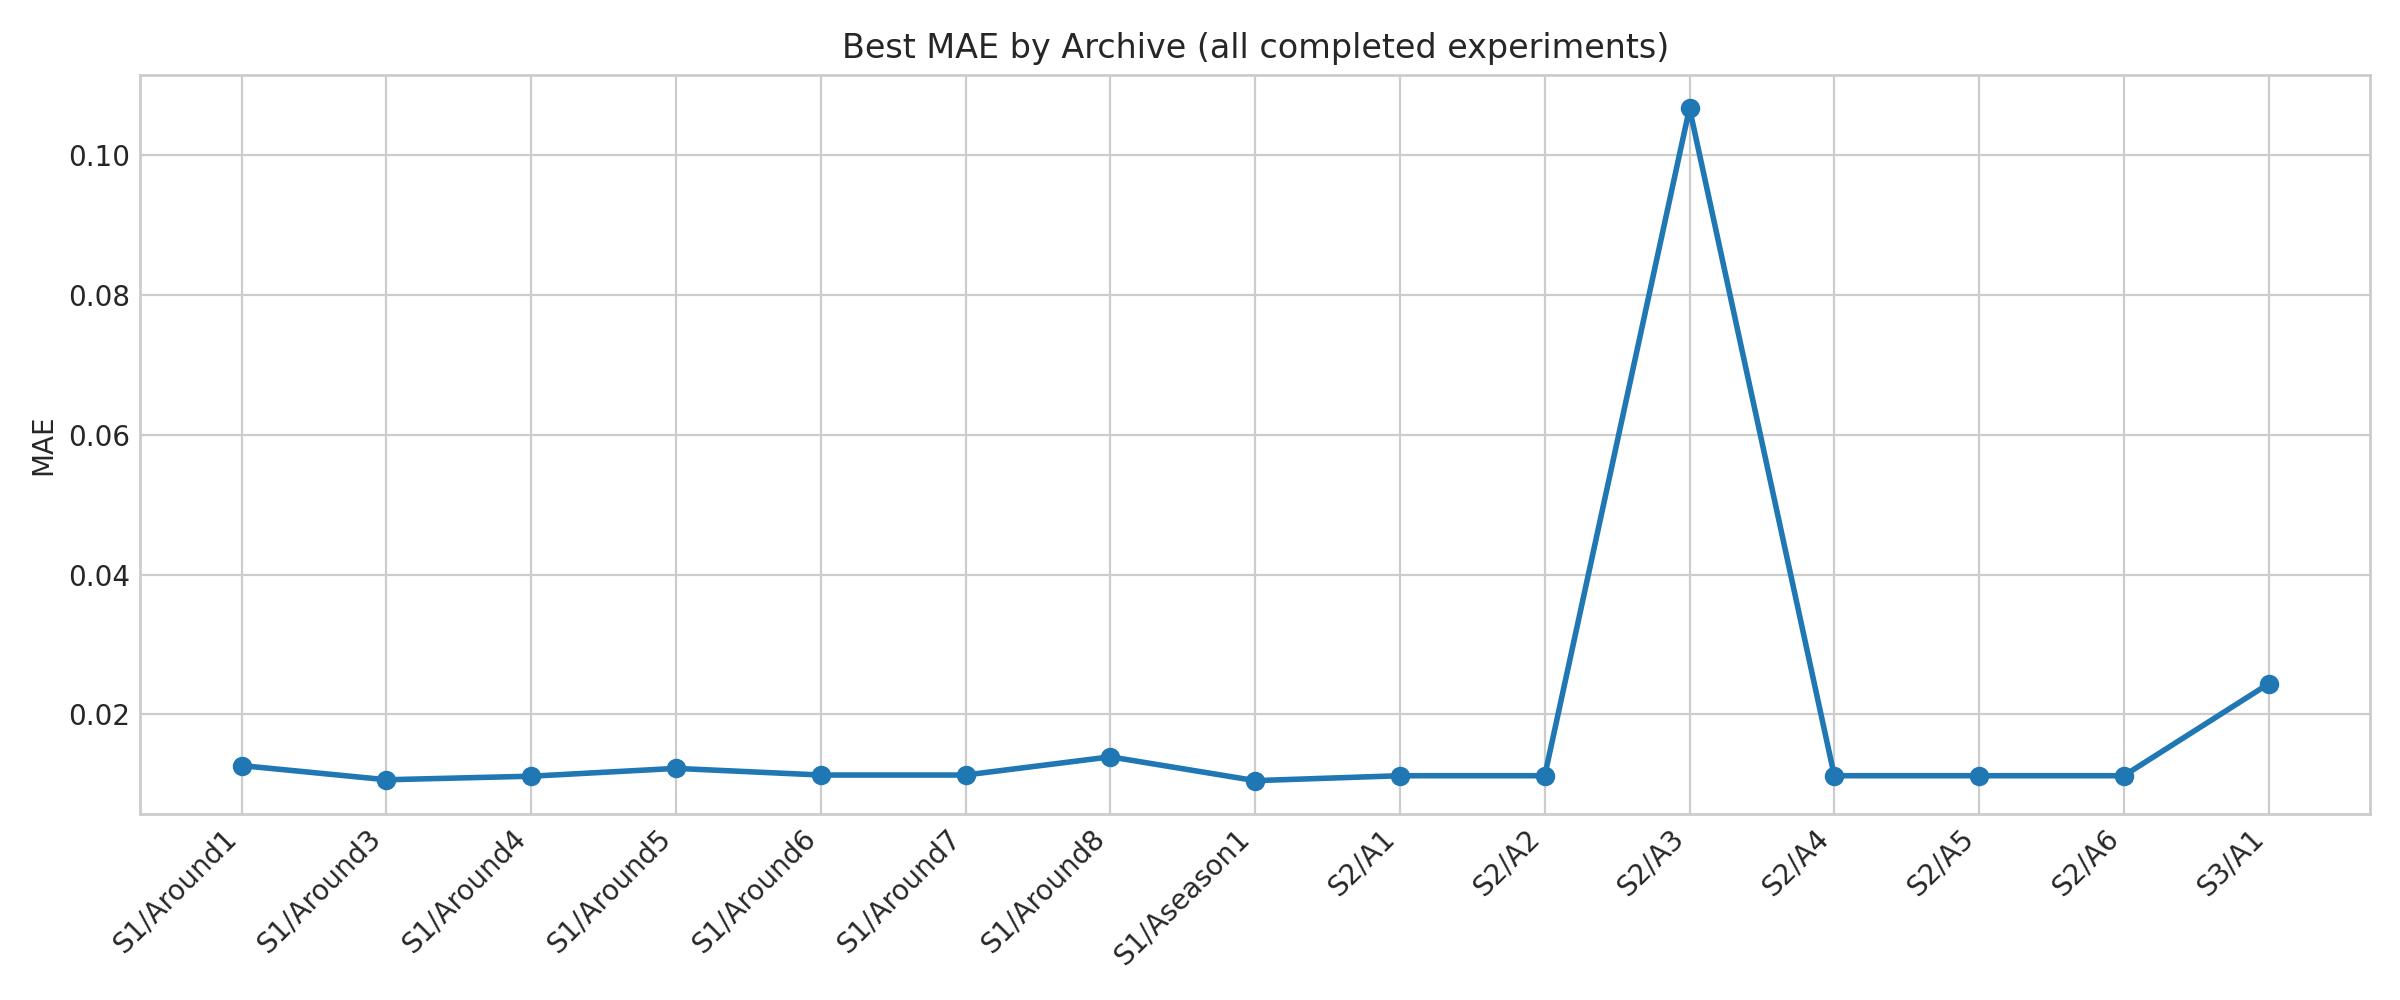
\includegraphics[width=0.92\linewidth]{archive_best_timeline_mae.png}
\caption{Best MAE by archive over the full project history. The season3 point should be read separately because its target protocol is different.}
\end{figure}

\subsection{Deployment-oriented reference models}

Table~\ref{tab:selected-models} collects the most important reference models for later reuse.

\begin{table}[H]
\centering
\small
\caption{Selected reference models for accuracy, deployability, and corrected-protocol benchmarking.}
\label{tab:selected-models}
\resizebox{\linewidth}{!}{%
\begin{tabular}{p{3.2cm} p{7.2cm} r r r p{3.4cm}}
\toprule
Role & Experiment & MAE & Params & Latency (ms) & Target \\
\midrule
Season2 best absolute & exp\_A5\_bodyframe\_plus\_imuint & 0.01125 & 409793 & 2.4362 & treadmill/left/speed\_leftbelt \\
Fusion best (old target) & exp\_S2A5\_B1\_fusion\_imuint & 0.01474 & 409892 & 2.5825 & treadmill/left/speed\_leftbelt \\
Dual+softprior & exp\_S2A6\_A4\_fusion\_dual\_softprior & 0.01860 & 410117 & 2.8162 & treadmill/left/speed\_leftbelt \\
Real-time fusion & exp\_S2A6\_B1\_fusion\_dual\_rt200 & 0.02154 & 143973 & 2.5941 & treadmill/left/speed\_leftbelt \\
Sensor-light & exp\_S2A6\_C2\_fusion\_imuint\_nogrf\_notorque & 0.02454 & 142364 & 2.627 & treadmill/left/speed\_leftbelt \\
Tiny Pareto & exp\_S2A6\_B3\_fusion\_dual\_tiny120 & 0.04026 & 74293 & 2.6813 & treadmill/left/speed\_leftbelt \\
Season3 corrected best & exp\_S3A1\_G009\_raw\_full\_w200\_base\_pglpf & 0.02439 & 409025 & 2.5932 & common/v\_Y\_true \\
Season3 corrected IMU-prior best & exp\_S3A1\_G079\_imuint\_full\_w200\_base\_none & 0.02442 & 409793 & 2.441 & common/v\_Y\_true \\
Season3 corrected fusion-lite & exp\_S3A1\_G130\_fusionimu\_lite\_w300\_compact\_none & 0.02603 & 142364 & 2.5662 & common/v\_Y\_true \\
Season3 corrected compact raw & exp\_S3A1\_G004\_raw\_full\_w300\_compact\_none & 0.02464 & 143153 & 2.5057 & common/v\_Y\_true \\
\bottomrule
\end{tabular}%
}

\end{table}

\subsection{Season3 archive\_1 top-20 under the corrected protocol}

The top-20 season3 runs are shown in Table~\ref{tab:s3-top20}. The top 10 all have detailed plots saved under \texttt{compare\_result/archive\_season3/archive\_1/...}.

\begin{table}[H]
\centering
\small
\caption{Season3 archive\_1 top-20 experiments under the corrected target protocol.}
\label{tab:s3-top20}
\resizebox{\linewidth}{!}{%
\begin{tabular}{r p{8.4cm} r r r r}
\toprule
Rank & Experiment & MAE & RMSE & Params & Latency (ms) \\
\midrule
1 & exp\_S3A1\_G009\_raw\_full\_w200\_base\_pglpf & 0.02439 & 0.03456 & 409025 & 2.5932 \\
2 & exp\_S3A1\_G079\_imuint\_full\_w200\_base\_none & 0.02442 & 0.03460 & 409793 & 2.441 \\
3 & exp\_S3A1\_G081\_imuint\_full\_w200\_base\_pglpf & 0.02452 & 0.03564 & 409793 & 2.4962 \\
4 & exp\_S3A1\_G004\_raw\_full\_w300\_compact\_none & 0.02464 & 0.03631 & 143153 & 2.5057 \\
5 & exp\_S3A1\_G130\_fusionimu\_lite\_w300\_compact\_none & 0.02603 & 0.03720 & 142364 & 2.5662 \\
6 & exp\_S3A1\_G062\_bf\_lite\_w200\_base\_glpf8 & 0.02622 & 0.03847 & 407681 & 2.4522 \\
7 & exp\_S3A1\_G110\_fusionimu\_full\_w300\_base\_glpf8 & 0.02622 & 0.03762 & 409892 & 2.5476 \\
8 & exp\_S3A1\_G014\_raw\_full\_w150\_base\_glpf8 & 0.02633 & 0.03742 & 409025 & 2.4754 \\
9 & exp\_S3A1\_G021\_raw\_lite\_w300\_base\_pglpf & 0.02636 & 0.03818 & 407105 & 2.4757 \\
10 & exp\_S3A1\_G063\_bf\_lite\_w200\_base\_pglpf & 0.02638 & 0.03914 & 407681 & 2.4403 \\
11 & exp\_S3A1\_G016\_raw\_full\_w150\_compact\_none & 0.02663 & 0.03821 & 143153 & 2.4097 \\
12 & exp\_S3A1\_G135\_fusionimu\_lite\_w200\_base\_pglpf & 0.02666 & 0.03803 & 407972 & 2.5974 \\
13 & exp\_S3A1\_G080\_imuint\_full\_w200\_base\_glpf8 & 0.02675 & 0.03815 & 409793 & 2.4461 \\
14 & exp\_S3A1\_G095\_imuint\_lite\_w300\_compact\_glpf8 & 0.02699 & 0.03935 & 142289 & 2.4399 \\
15 & exp\_S3A1\_G145\_dual\_full\_w300\_base\_none & 0.02708 & 0.03949 & 410117 & 2.6729 \\
16 & exp\_S3A1\_G129\_fusionimu\_lite\_w300\_base\_pglpf & 0.02708 & 0.03956 & 407972 & 2.5926 \\
17 & exp\_S3A1\_G097\_imuint\_lite\_w200\_base\_none & 0.02719 & 0.03936 & 407873 & 2.4502 \\
18 & exp\_S3A1\_G146\_dual\_full\_w300\_base\_glpf8 & 0.02737 & 0.03927 & 410117 & 2.7391 \\
19 & exp\_S3A1\_G055\_bf\_lite\_w300\_base\_none & 0.02765 & 0.04136 & 407681 & 2.4712 \\
20 & exp\_S3A1\_G022\_raw\_lite\_w300\_compact\_none & 0.02769 & 0.04113 & 141113 & 2.3401 \\
\bottomrule
\end{tabular}%
}

\end{table}

\begin{figure}[H]
\centering
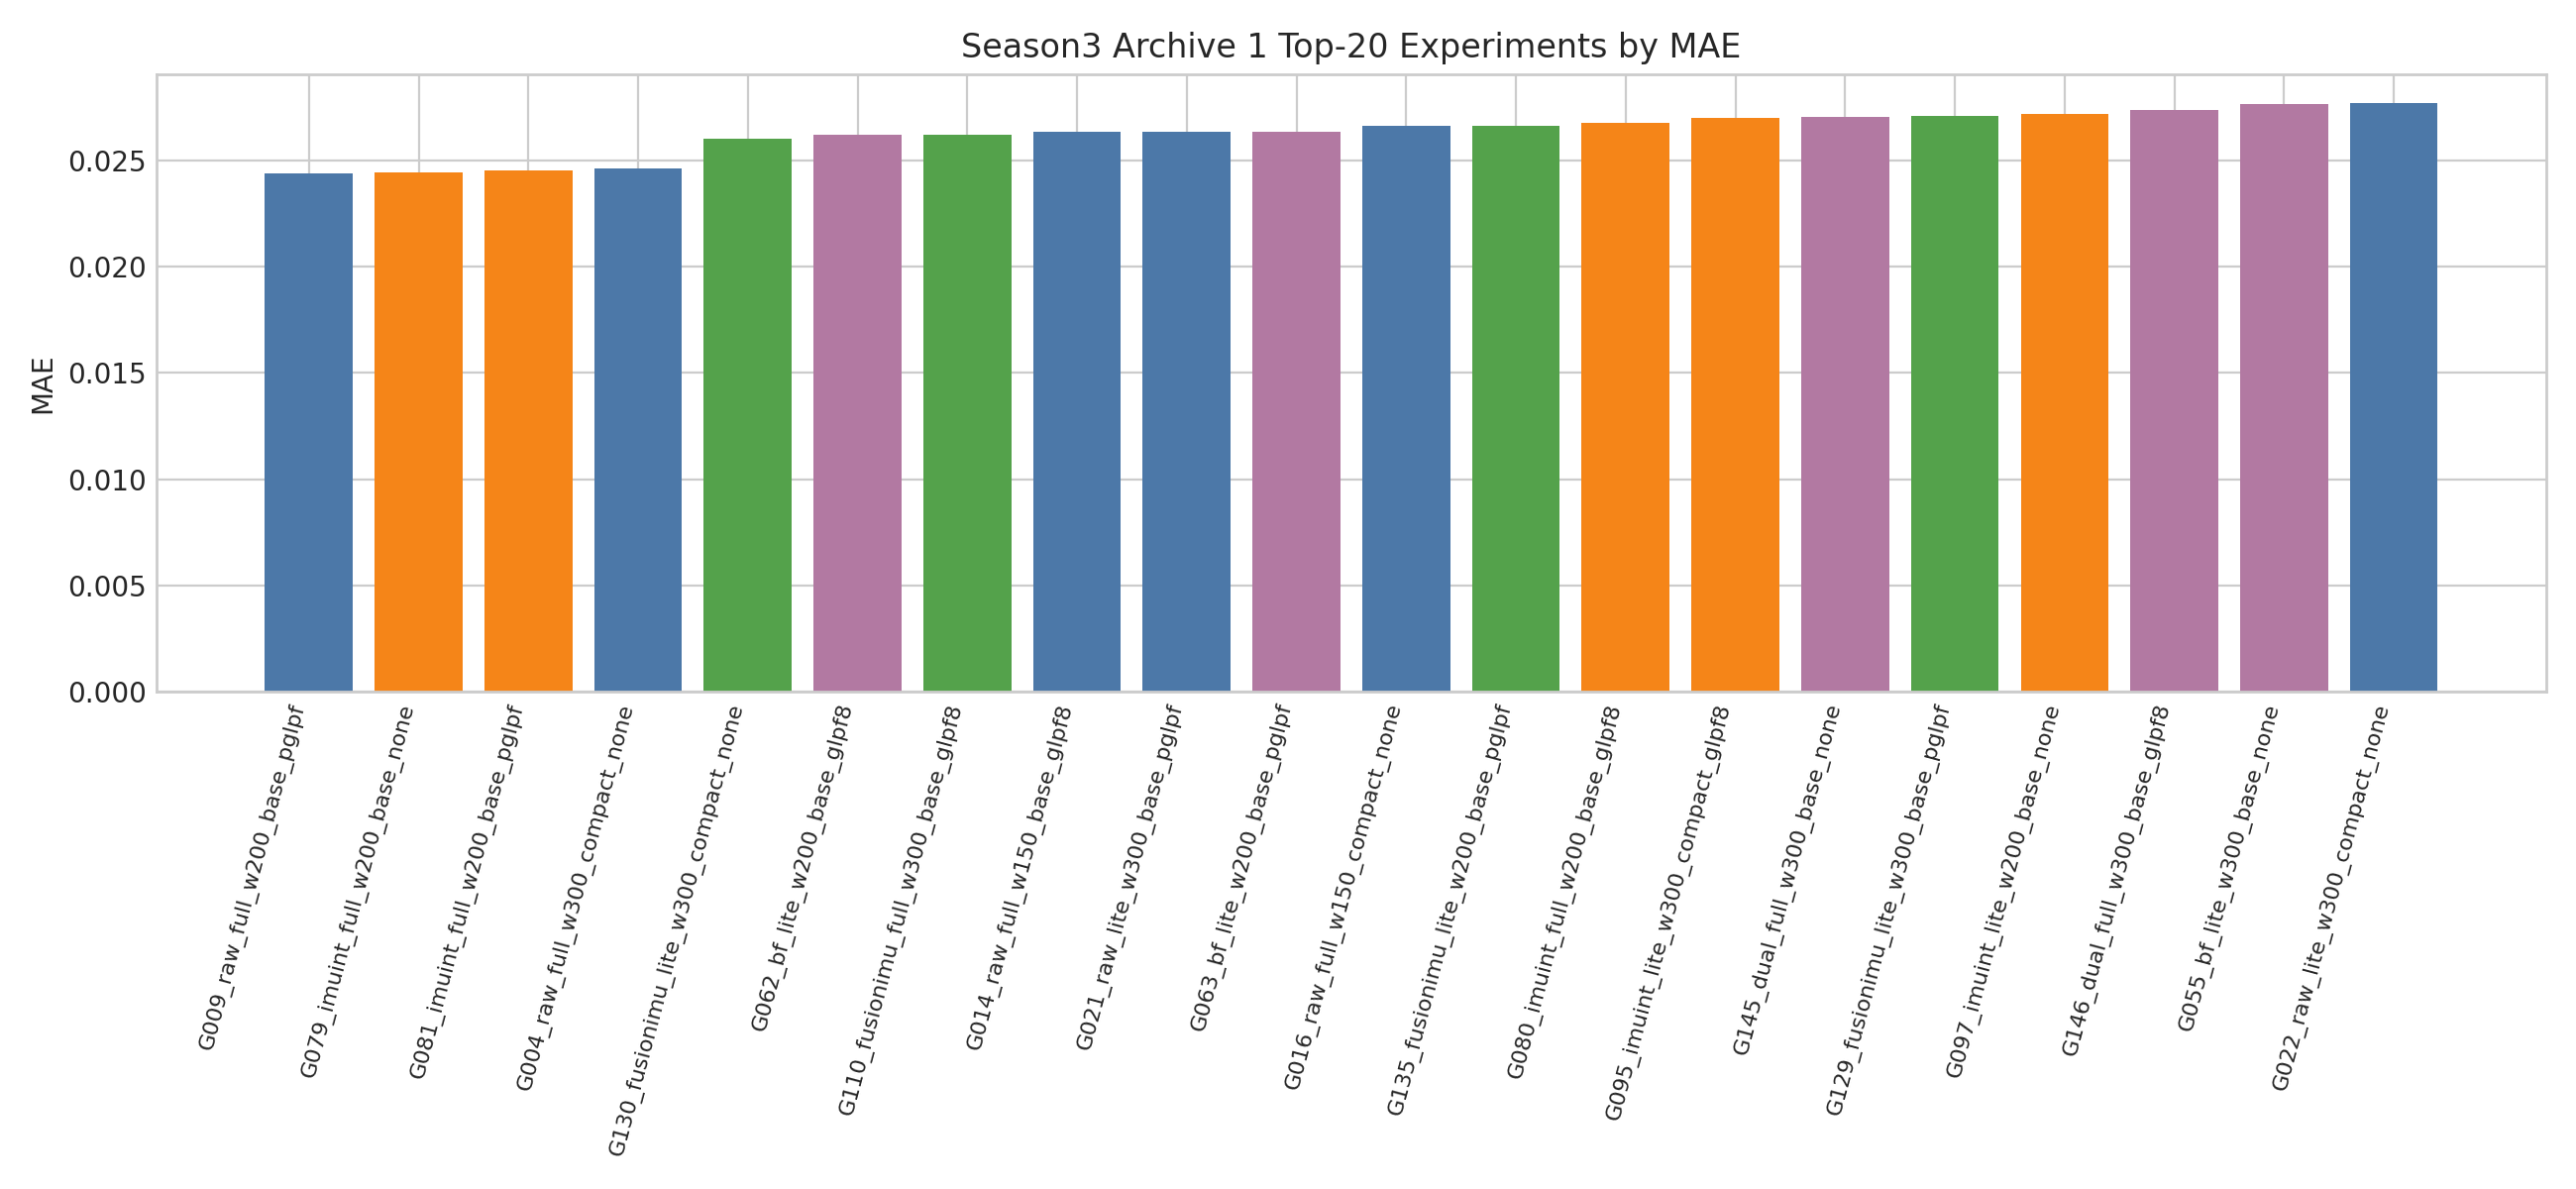
\includegraphics[width=0.97\linewidth]{season3_top20_mae.png}
\caption{Season3 archive\_1 top-20 runs by MAE. The very top of the ranking is dominated by raw\_full and imuint\_full variants.}
\end{figure}

\subsection{Season3 family-level summary}

\begin{table}[H]
\centering
\small
\caption{Best season3 experiment from each major family.}
\resizebox{\linewidth}{!}{%
\begin{tabular}{p{2.8cm} p{8.0cm} r r r}
\toprule
Family & Best experiment & MAE & RMSE & Params \\
\midrule
raw\_full & exp\_S3A1\_G009\_raw\_full\_w200\_base\_pglpf & 0.02439 & 0.03456 & 409025 \\
imuint\_full & exp\_S3A1\_G079\_imuint\_full\_w200\_base\_none & 0.02442 & 0.03460 & 409793 \\
fusionimu\_lite & exp\_S3A1\_G130\_fusionimu\_lite\_w300\_compact\_none & 0.02603 & 0.03720 & 142364 \\
bf\_lite & exp\_S3A1\_G062\_bf\_lite\_w200\_base\_glpf8 & 0.02622 & 0.03847 & 407681 \\
fusionimu\_full & exp\_S3A1\_G110\_fusionimu\_full\_w300\_base\_glpf8 & 0.02622 & 0.03762 & 409892 \\
raw\_lite & exp\_S3A1\_G021\_raw\_lite\_w300\_base\_pglpf & 0.02636 & 0.03818 & 407105 \\
imuint\_lite & exp\_S3A1\_G095\_imuint\_lite\_w300\_compact\_glpf8 & 0.02699 & 0.03935 & 142289 \\
dual\_full & exp\_S3A1\_G145\_dual\_full\_w300\_base\_none & 0.02708 & 0.03949 & 410117 \\
bf\_full & exp\_S3A1\_G039\_bf\_full\_w300\_base\_pglpf & 0.02806 & 0.04161 & 409601 \\
dualsoft\_full & exp\_S3A1\_G172\_dualsoft\_full\_w200\_compact\_none & 0.02886 & 0.04039 & 143973 \\
\bottomrule
\end{tabular}%
}

\end{table}

\begin{figure}[H]
\centering
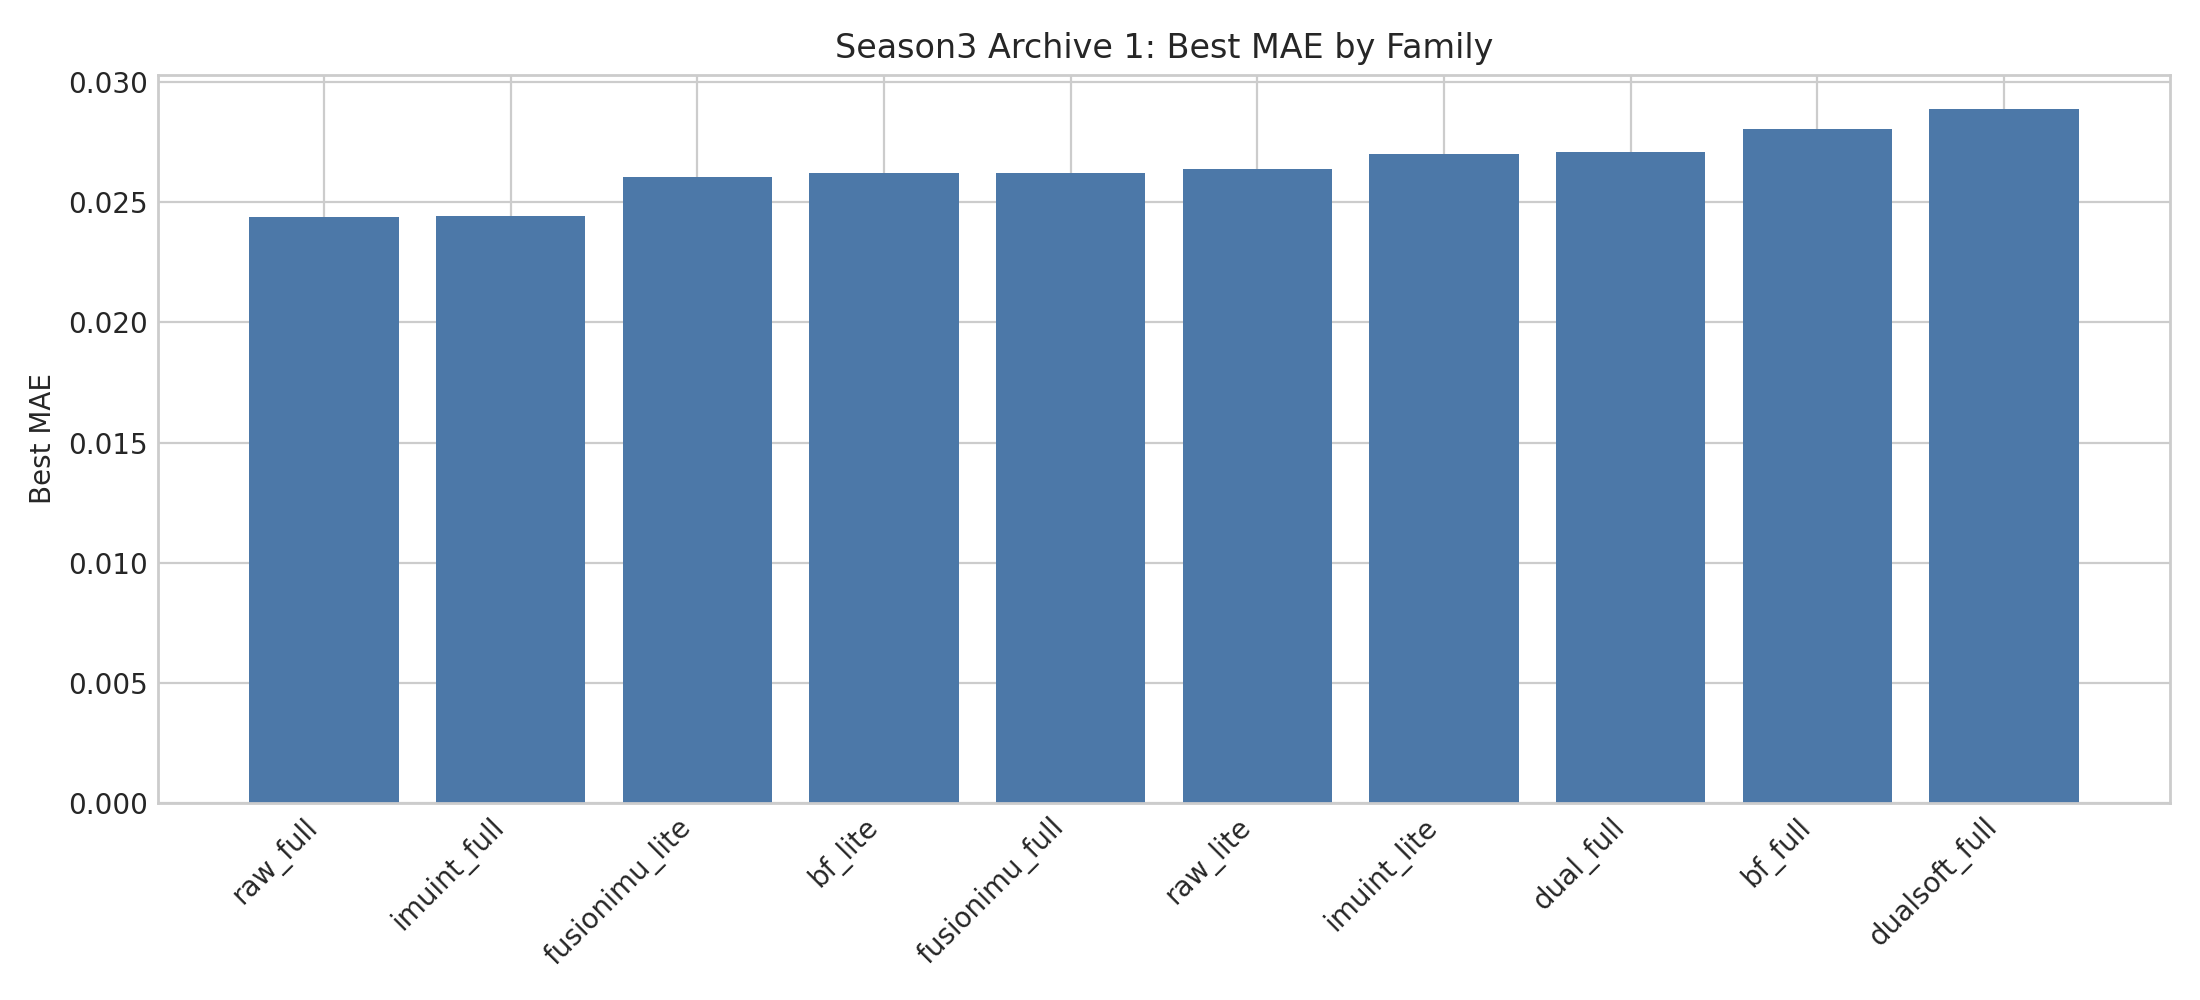
\includegraphics[width=0.90\linewidth]{season3_family_best_mae.png}
\caption{Best MAE achieved by each family in season3 archive\_1.}
\end{figure}

\section{Interpretation of the Main Results}

\subsection{What remained true after the target was corrected}

Some conclusions survived the protocol change:

\begin{itemize}
\item \texttt{imu\_integrated\_speed} remained a strong prior.
\item 200-frame context was a very good operating point.
\item compact models could come surprisingly close to the full-size baseline.
\item causal TCN+GRU models remained a strong default.
\end{itemize}

\subsection{What changed after the target was corrected}

The biggest shift was representational:

\begin{itemize}
\item under season2's old protocol, the body-frame + IMU-prior baseline looked dominant,
\item under season3's corrected protocol, \texttt{raw\_full} and \texttt{imuint\_full} moved to the top,
\item fusion remained competitive but became a near-best alternative rather than the absolute best.
\end{itemize}

The season3 top 5 makes this explicit:

\begin{enumerate}
\item \texttt{exp\_S3A1\_G009\_raw\_full\_w200\_base\_pglpf}: MAE 0.02439
\item \texttt{exp\_S3A1\_G079\_imuint\_full\_w200\_base\_none}: MAE 0.02442
\item \texttt{exp\_S3A1\_G081\_imuint\_full\_w200\_base\_pglpf}: MAE 0.02452
\item \texttt{exp\_S3A1\_G004\_raw\_full\_w300\_compact\_none}: MAE 0.02464
\item \texttt{exp\_S3A1\_G130\_fusionimu\_lite\_w300\_compact\_none}: MAE 0.02603
\end{enumerate}

\subsection{Why the fusion story is still useful}

Even though fusion is not the best corrected-protocol family in absolute MAE, it still matters because:

\begin{itemize}
\item it remains close to the top,
\item it is structurally interpretable,
\item it gives a clean ``learned branch + physics prior'' deployment story,
\item compact fusion models are promising when sensor count or model size matters.
\end{itemize}

\subsection{Sensor-light and tiny models remain valuable}

Some season2 archive\_6 models are still highly valuable for practical deployment studies:

\begin{itemize}
\item \texttt{exp\_S2A6\_C2\_fusion\_imuint\_nogrf\_notorque} removes both GRF and exoskeleton torques,
\item \texttt{exp\_S2A6\_B3\_fusion\_dual\_tiny120} demonstrates a much smaller network,
\item \texttt{exp\_S3A1\_G004\_raw\_full\_w300\_compact\_none} shows that corrected-protocol compact raw models can remain highly competitive.
\end{itemize}

\section{Representative Qualitative Plots}

\subsection{Best corrected-protocol raw model}

\begin{figure}[H]
\centering
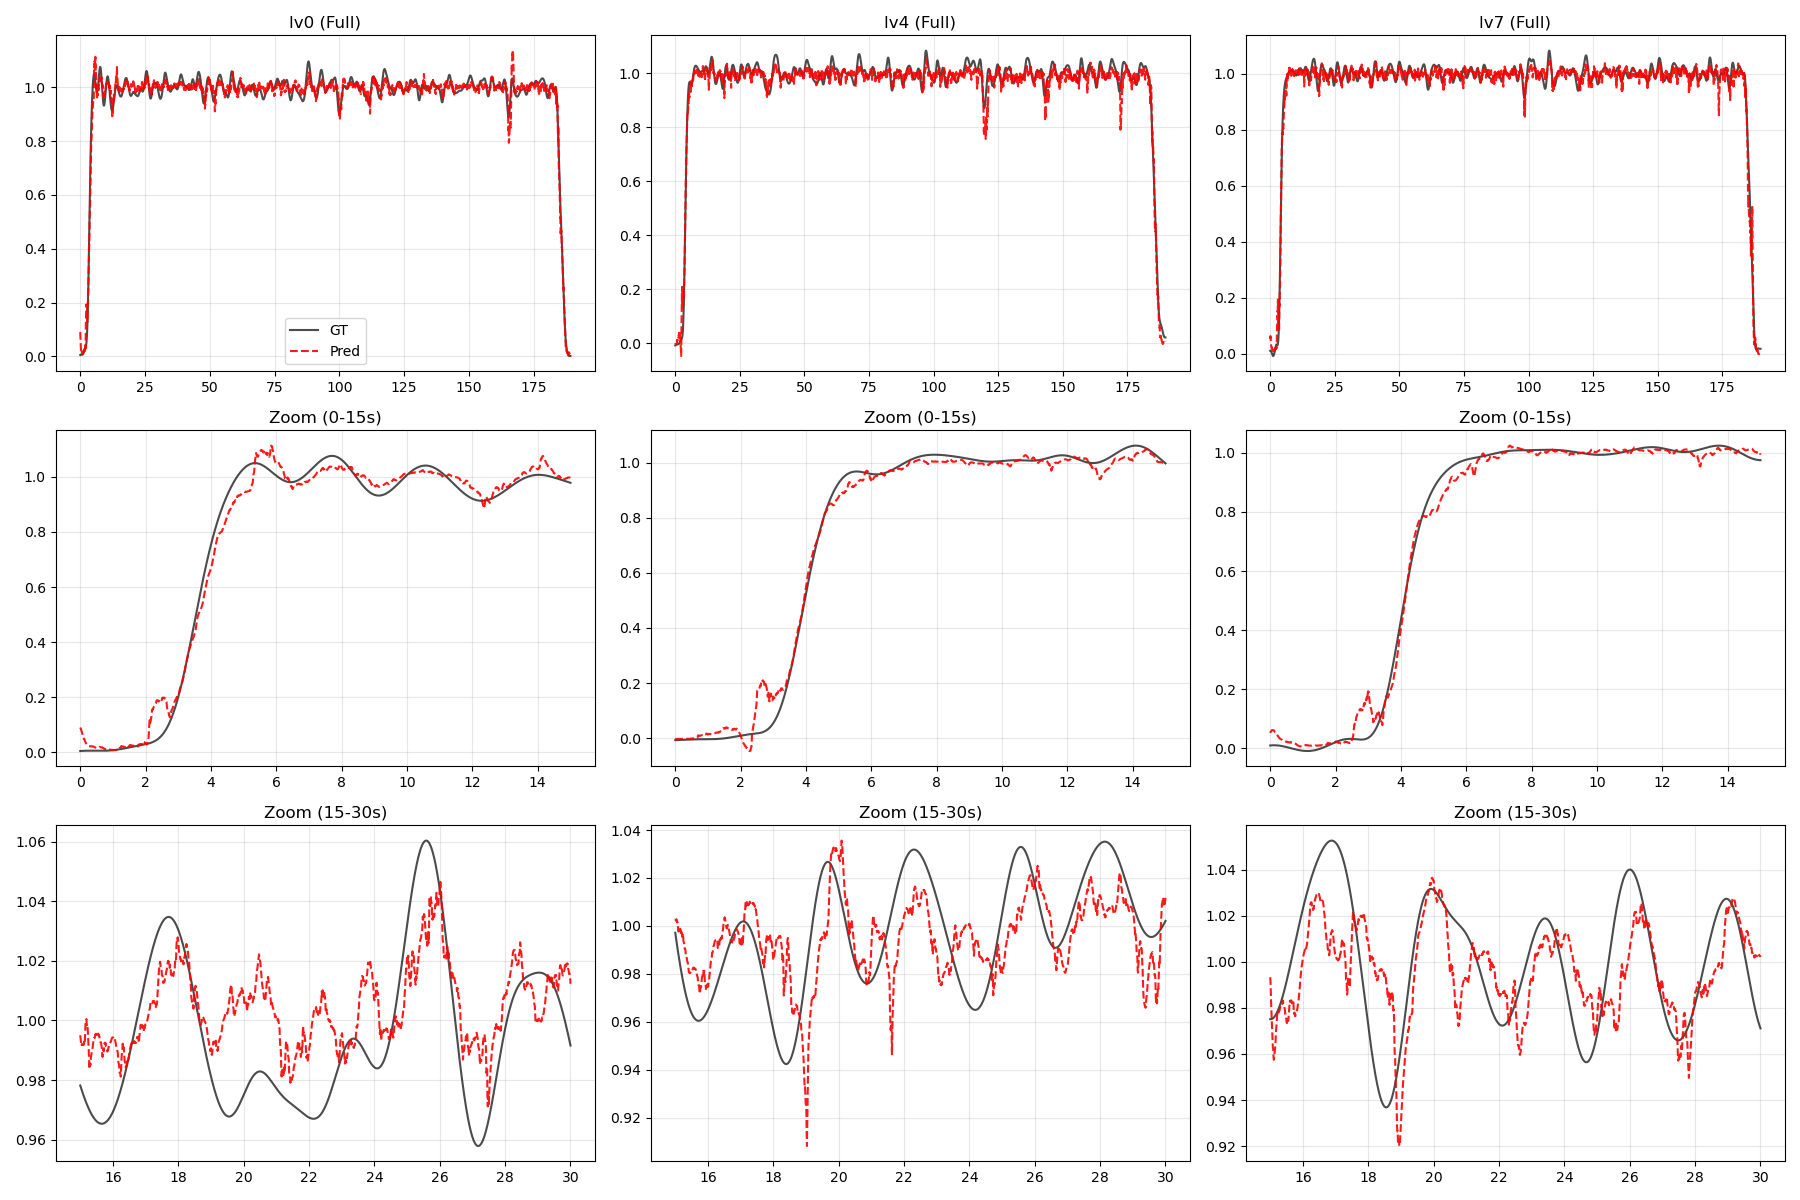
\includegraphics[width=0.95\linewidth]{s3_g009_level100.png}
\caption{Season3 best raw model on \texttt{level\_100mps}: \texttt{exp\_S3A1\_G009\_raw\_full\_w200\_base\_pglpf}.}
\end{figure}

\begin{figure}[H]
\centering
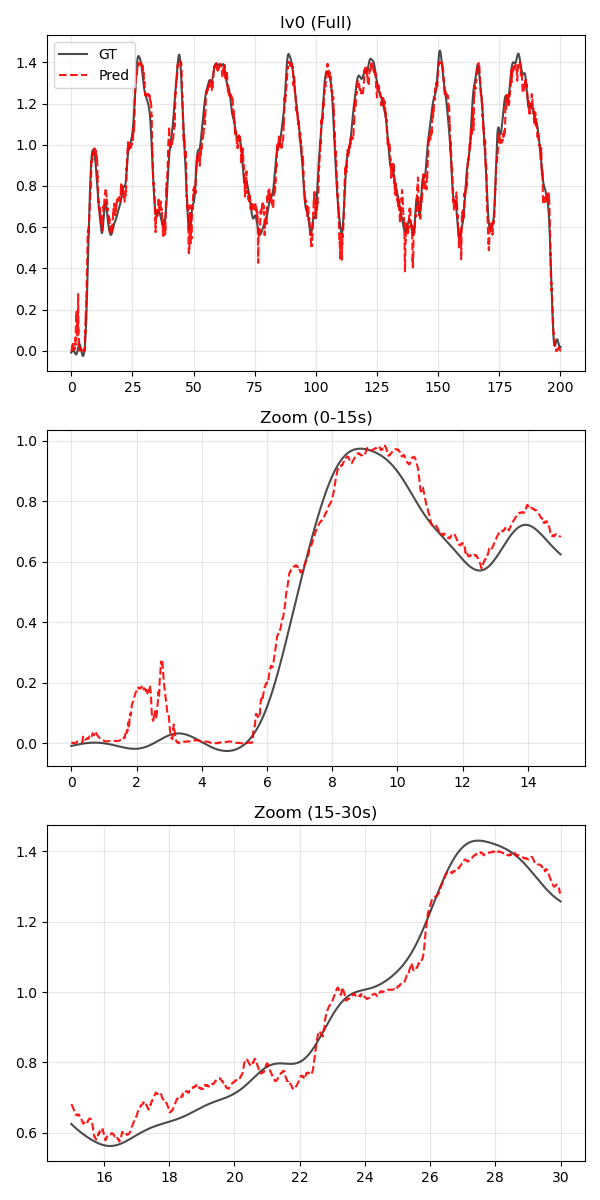
\includegraphics[width=0.95\linewidth]{s3_g009_accel_sine.png}
\caption{Season3 best raw model on \texttt{accel\_sine}.}
\end{figure}

\subsection{Best corrected-protocol IMU-prior model}

\begin{figure}[H]
\centering
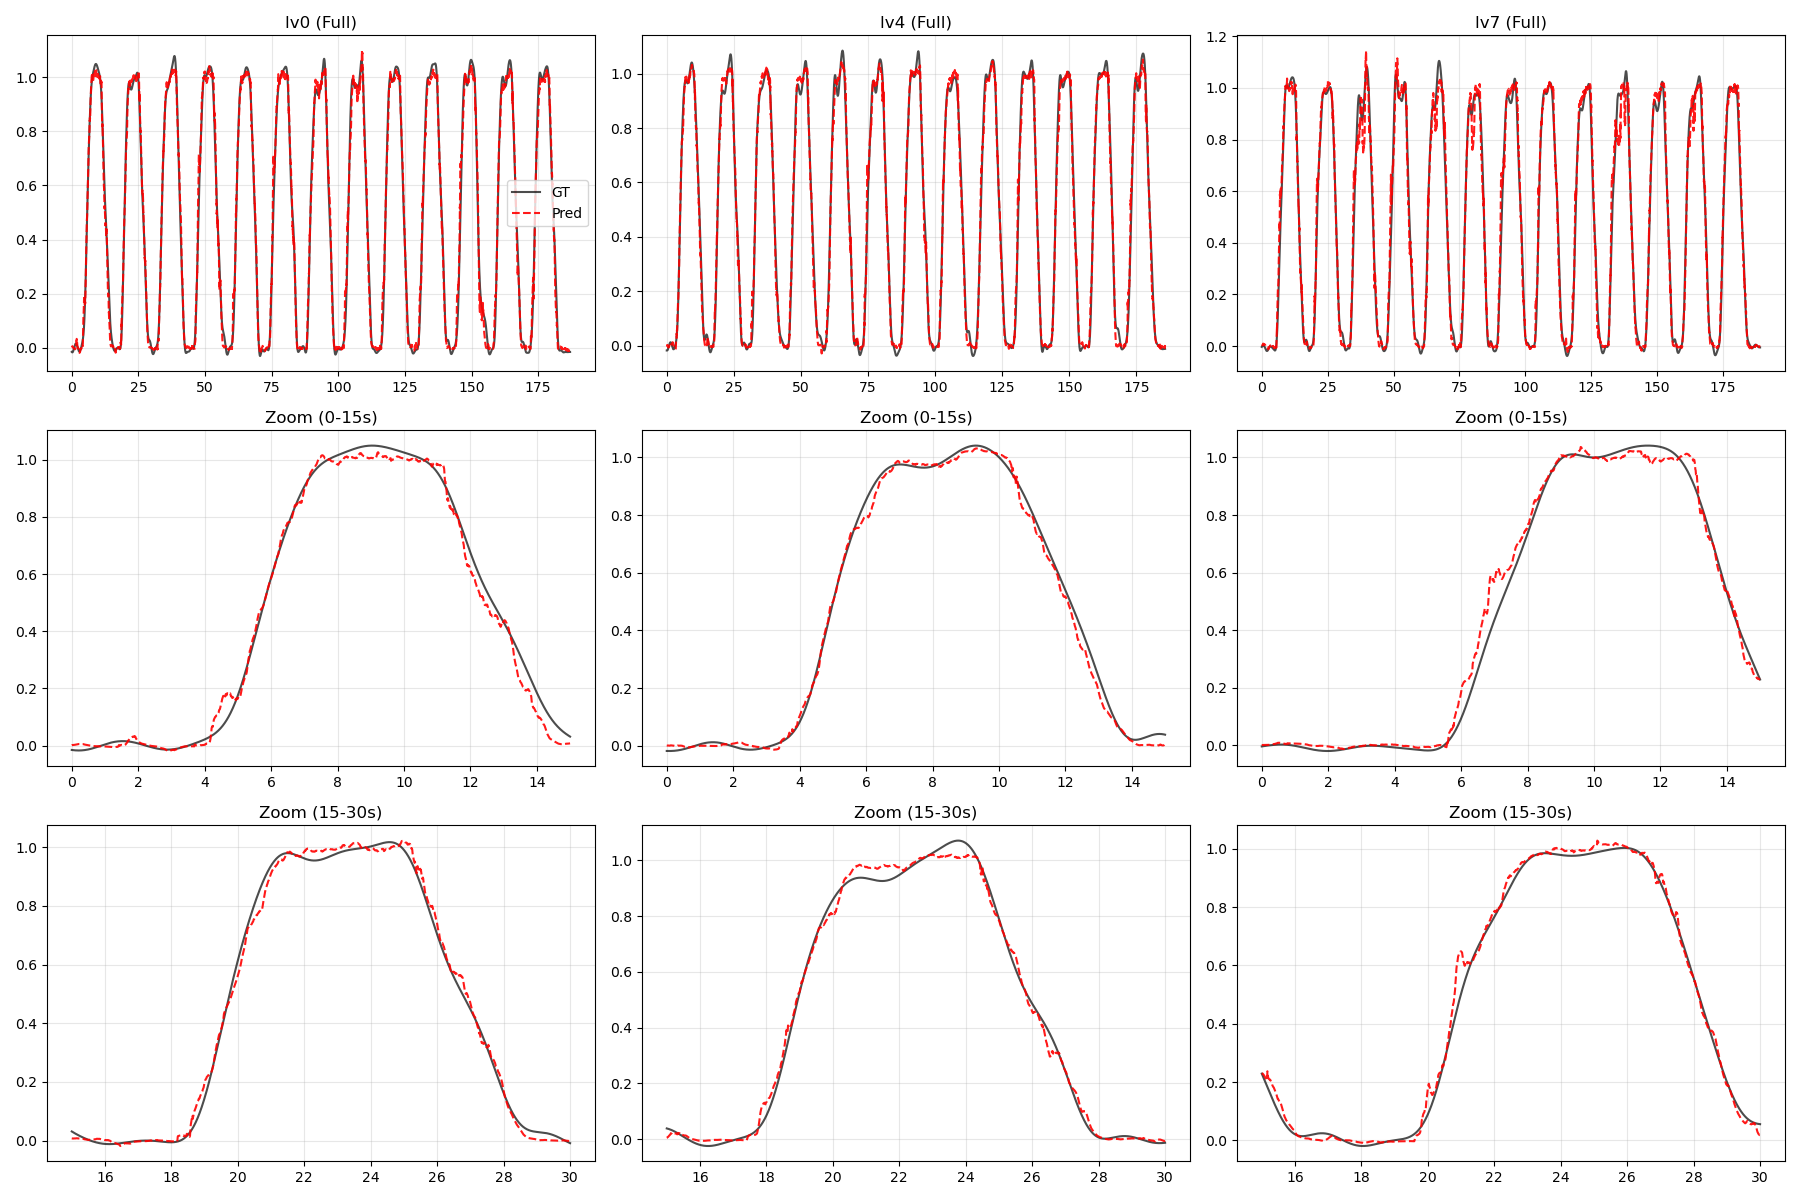
\includegraphics[width=0.95\linewidth]{s3_g079_stopandgo.png}
\caption{Season3 best IMU-prior model on \texttt{stopandgo}: \texttt{exp\_S3A1\_G079\_imuint\_full\_w200\_base\_none}.}
\end{figure}

\subsection{Representative compact fusion model}

\begin{figure}[H]
\centering
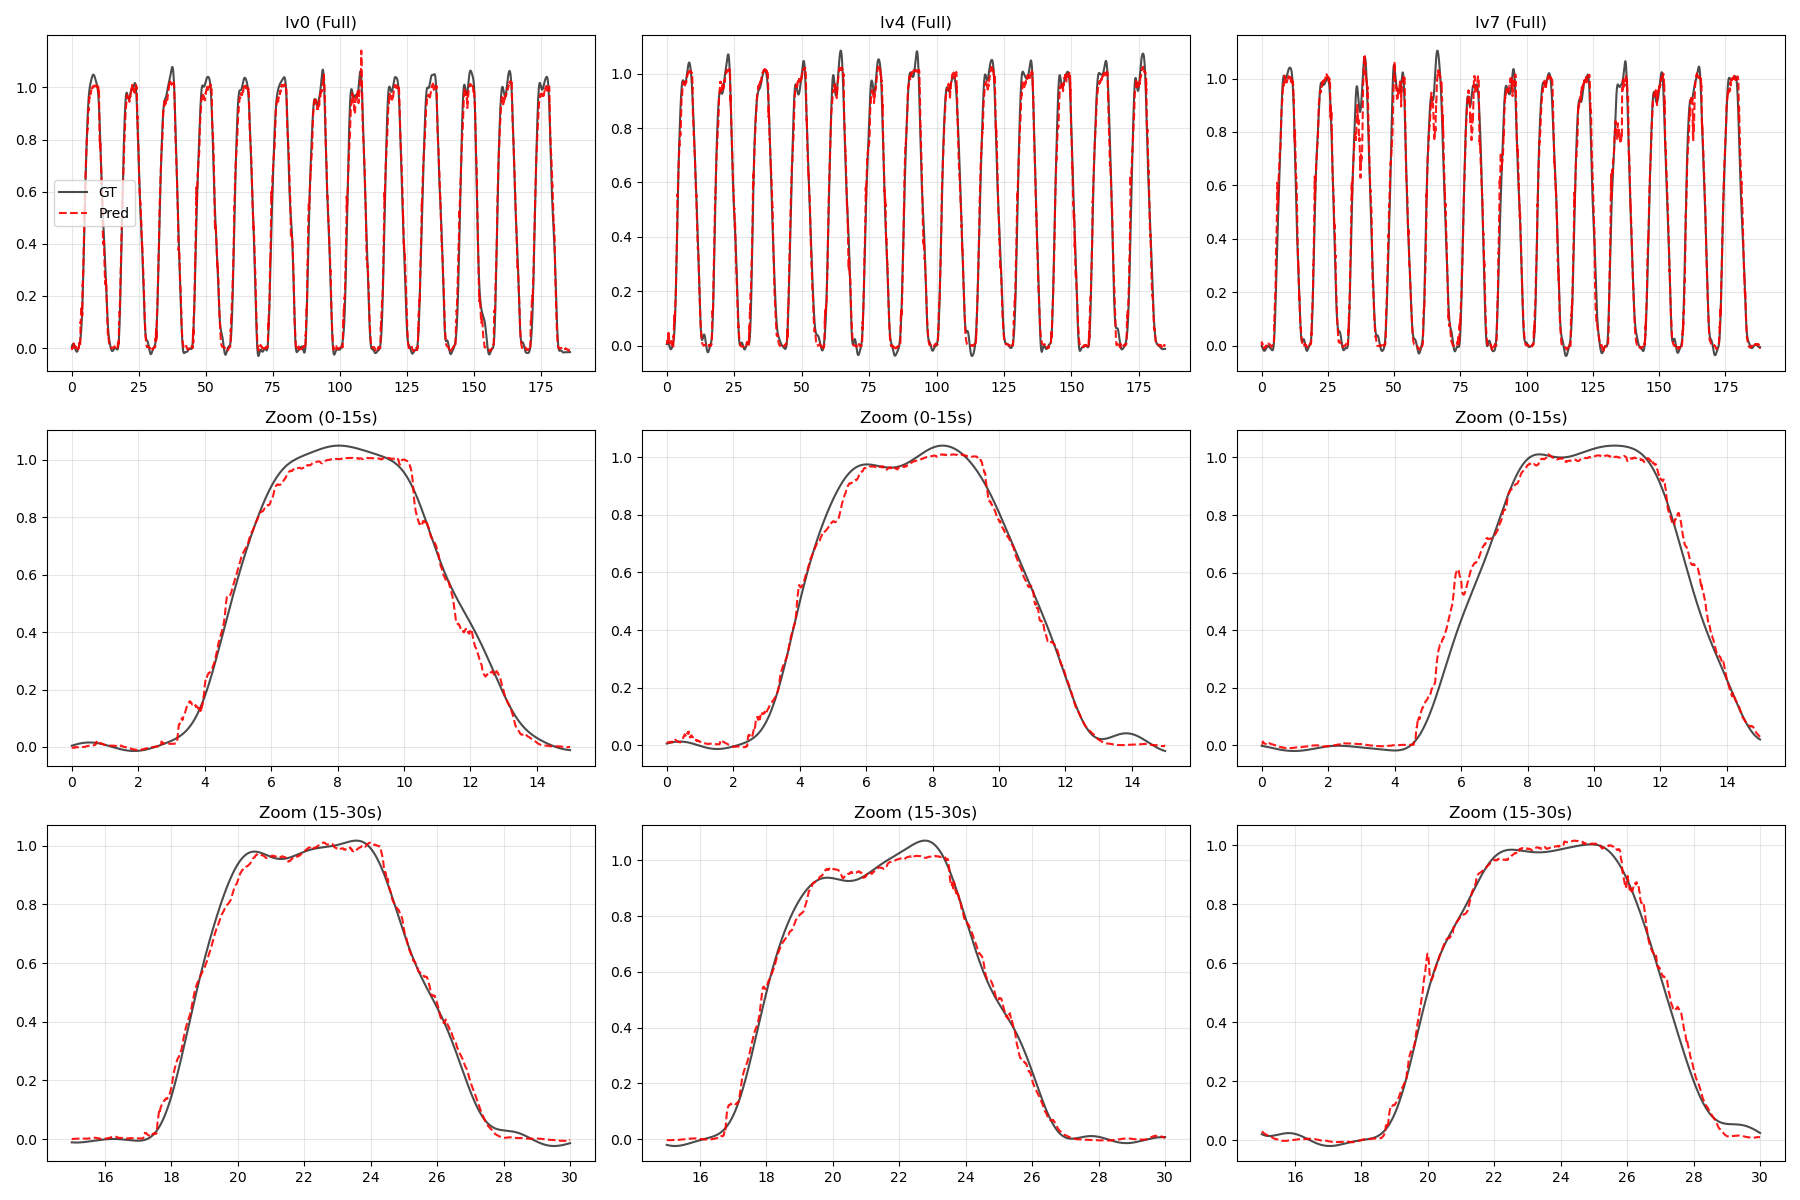
\includegraphics[width=0.95\linewidth]{s3_g130_stopandgo.png}
\caption{Compact fusion model on \texttt{stopandgo}: \texttt{exp\_S3A1\_G130\_fusionimu\_lite\_w300\_compact\_none}.}
\end{figure}

\subsection{Training curves}

\begin{figure}[H]
\centering
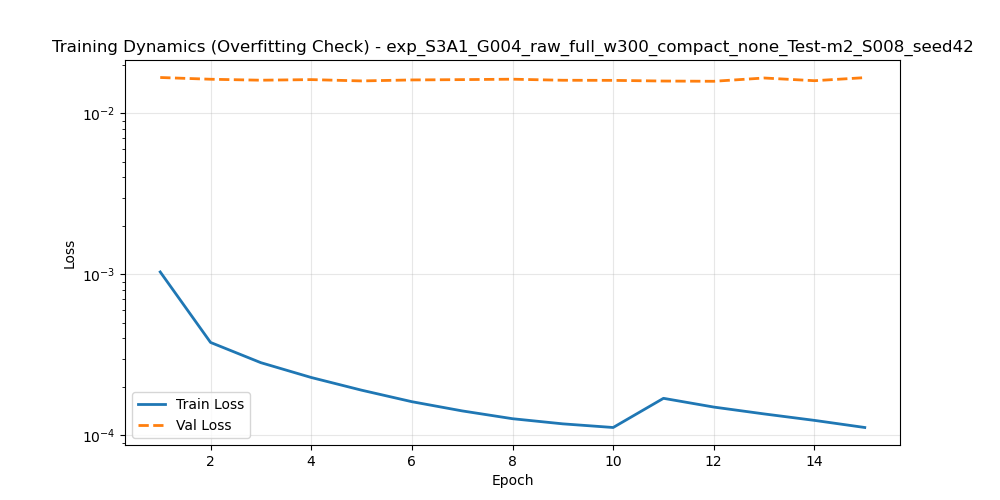
\includegraphics[width=0.86\linewidth]{s3_g004_training_curves.png}
\caption{Training curves for the best compact raw season3 model.}
\end{figure}

\begin{figure}[H]
\centering
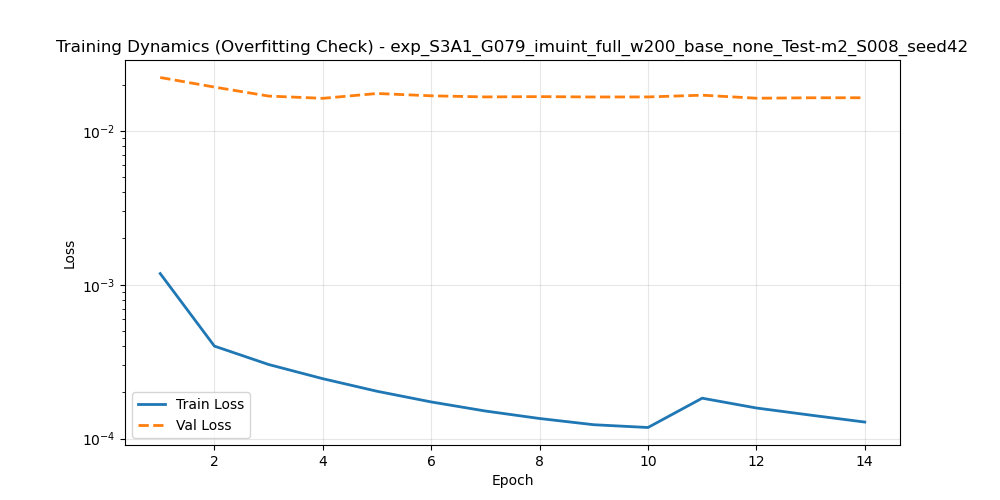
\includegraphics[width=0.86\linewidth]{s3_g079_training_curves.png}
\caption{Training curves for the best corrected-protocol IMU-prior model.}
\end{figure}

\section{Feature Importance and Interpretability}

The repository supports permutation feature importance through \texttt{compare\_results.py}. In practice, this path was more stable in the old protocol than in the late season3 sweep. The most reliable feature-importance artifact currently available in the repository is the season1 asset shown below.

\begin{figure}[H]
\centering
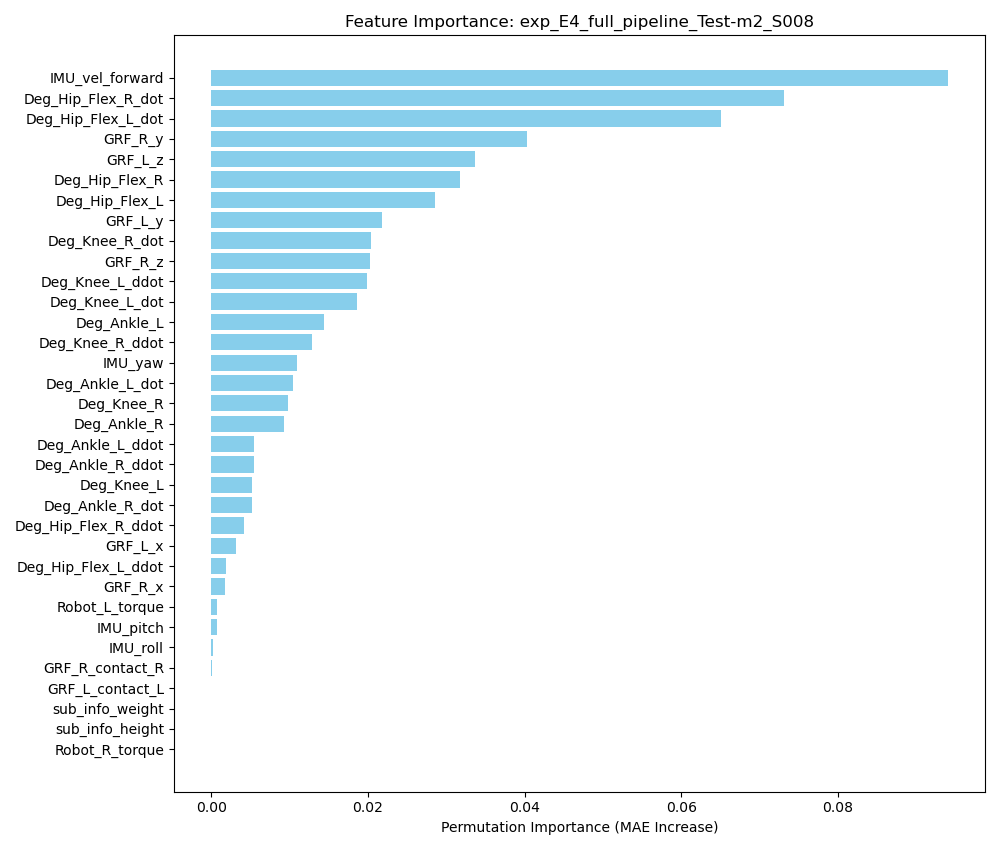
\includegraphics[width=0.82\linewidth]{season1_feature_importance_best.png}
\caption{Representative feature-importance output from the old-protocol phase of the project. Later season3 plot generation succeeded, but the feature-importance tail of the evaluation script still needs cleanup for fully reliable cross-archive use.}
\end{figure}

Interpretability findings from the experimental history are more robust than the raw feature-importance plots:

\begin{itemize}
\item IMU-integrated speed is a meaningful and repeatedly helpful prior.
\item Model-based COM speed is physically appealing but less consistently useful than the IMU prior.
\item Body-frame IMU helped strongly under the old protocol, but its advantage was reduced under the corrected protocol.
\item Raw kinematics remain extremely strong.
\end{itemize}

\section{Compute Burden and Real-Time Feasibility}

\subsection{Model-side compute burden}

Most representative models sit in one of three ranges:

\begin{itemize}
\item \textbf{full models:} about 407k--410k parameters
\item \textbf{compact models:} about 142k--143k parameters
\item \textbf{tiny models:} about 74k parameters
\end{itemize}

Host-side latency for representative deployed forward passes was typically about 2.4--2.6\,ms in the saved metrics, although this number is sensitive to measurement conditions and should not be over-interpreted at sub-millisecond precision.

\subsection{Preprocessing-side compute burden}

Real-time feasibility depends on more than the neural model. The preprocessing burden varies by family:

\begin{itemize}
\item \textbf{raw families:} lightest derived-feature burden; mostly raw kinematics, raw IMU orientation features, and simple contact/torque handling.
\item \textbf{body-frame families:} require quaternion processing, gravity removal, and causal forward-axis estimation.
\item \textbf{imuint families:} add leaky integration and causal LPF, which are lightweight and online-feasible.
\item \textbf{model\_com/dual families:} require more kinematic prior computation and stance logic.
\item \textbf{sensor-light variants:} reduce both hardware and preprocessing complexity by removing GRF and/or torque inputs.
\end{itemize}

From a deployment perspective, the most attractive candidates are therefore:

\begin{itemize}
\item season2 sensor-light fusion models,
\item season2 tiny Pareto models,
\item season3 compact raw or compact fusion models.
\end{itemize}

\begin{figure}[H]
\centering
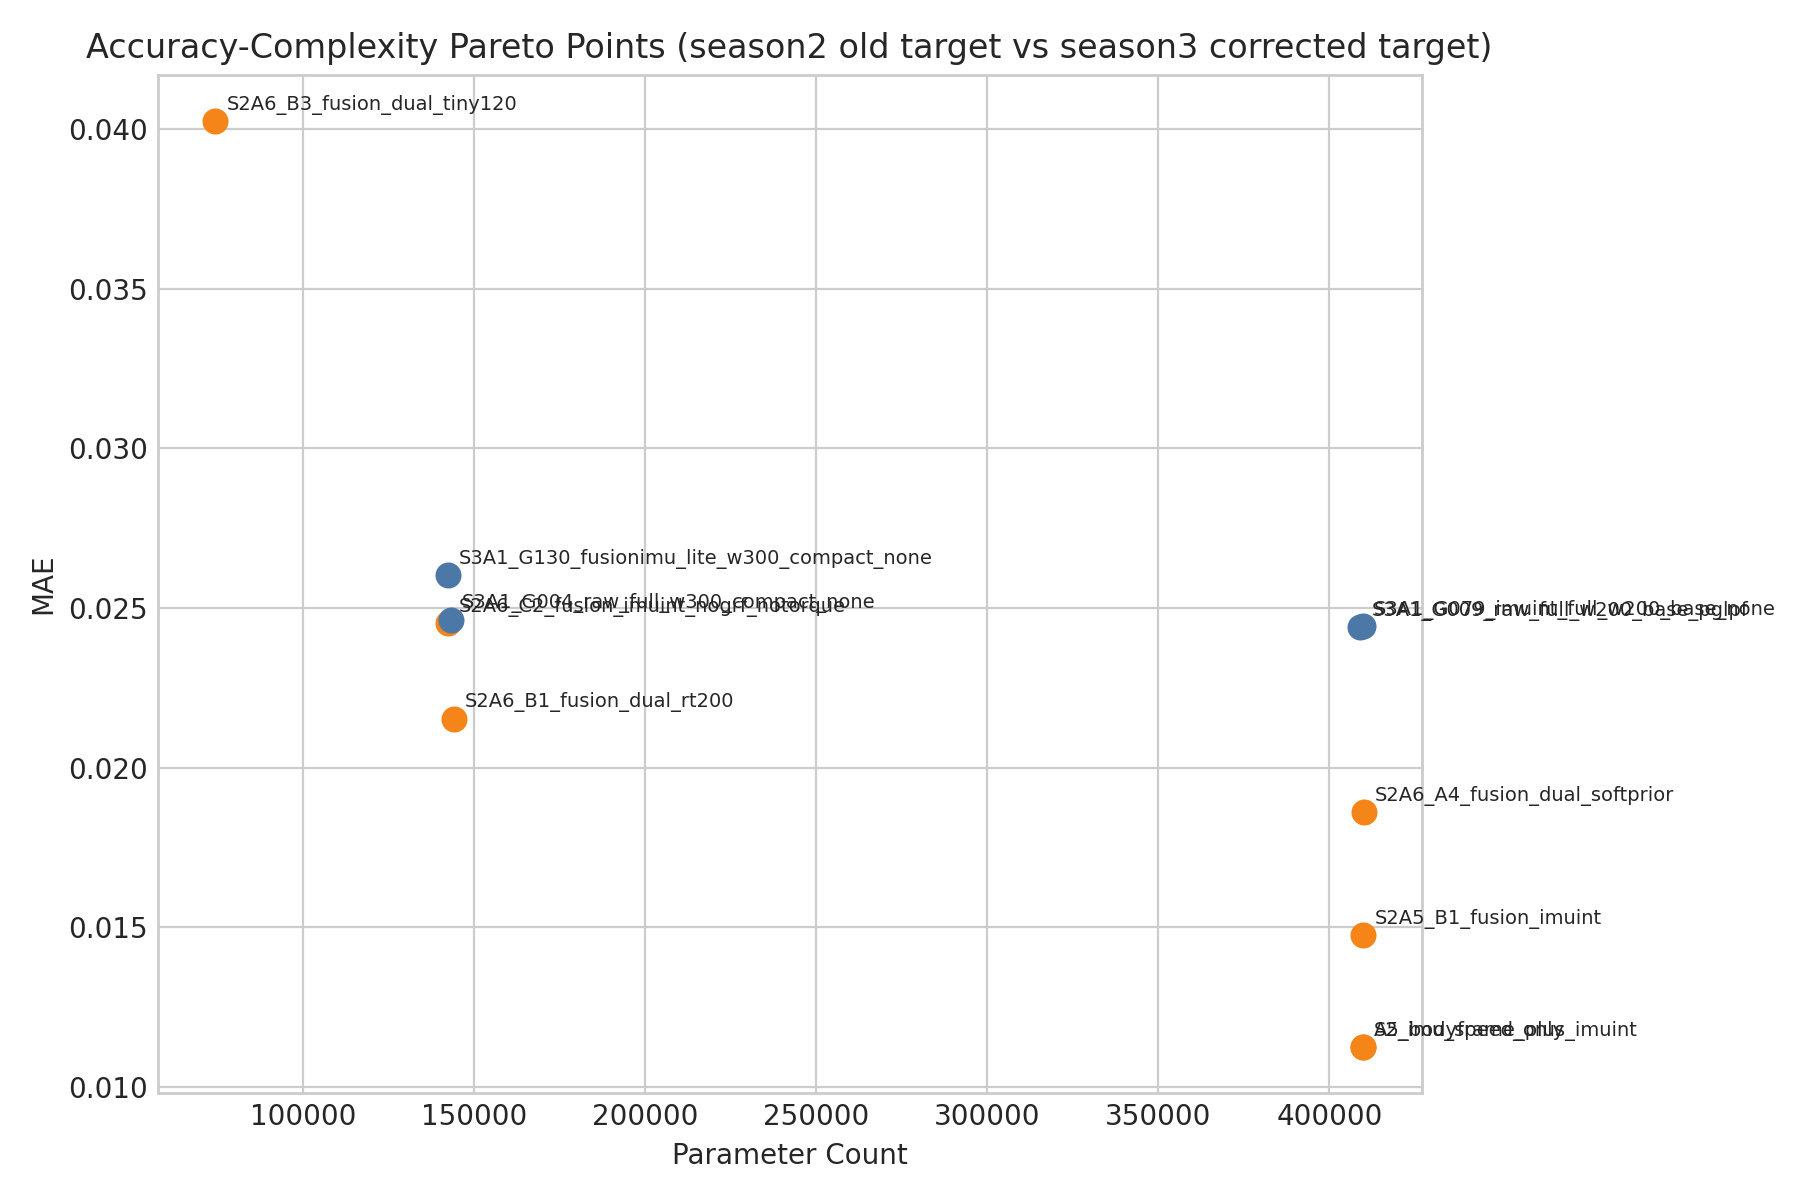
\includegraphics[width=0.90\linewidth]{overall_pareto_params_mae.png}
\caption{Selected Pareto points across old-protocol and corrected-protocol phases. This figure is most useful for understanding tradeoff structure, not for making direct cross-protocol ranking claims.}
\end{figure}

\subsection{Evaluation-side compute burden}

Evaluation was often more computationally awkward than training because plotting and detailed analysis were CPU- and memory-heavy. Several practical lessons emerged:

\begin{itemize}
\item permutation feature importance should be run separately from fast metric screening,
\item full trajectory/detailed plots are better limited to a small top-\(k\) subset,
\item \texttt{EVAL\_STRIDE=3} was a useful compromise for first-pass evaluation,
\item detailed evaluation originally caused repeated memory failures until the batching and concatenation path was fixed.
\end{itemize}

\section{What Worked, What Failed, and What to Reuse}

\subsection{Strongest positive findings}

\begin{itemize}
\item Under the old protocol, body-frame IMU plus IMU-integrated speed was the strongest overall baseline.
\item IMU-integrated speed was consistently more helpful than model-based COM speed.
\item Confidence-weighted fusion was the only later ``new family'' that repeatedly showed positive signal.
\item Compact and sensor-light models created credible practical tradeoffs even when they did not beat the strongest full baseline.
\item Under the corrected protocol, raw\_full and imuint\_full families emerged as the strongest top-line performers.
\end{itemize}

\subsection{Repeated negative findings}

\begin{itemize}
\item Hard residual skip was unstable and generally unsuccessful.
\item Observer-style propagated priors did not work well.
\item Distillation did not produce a reliable improvement.
\item Model-based COM speed was usually not the main performance driver.
\item Bigger structural changes such as multiscale or smoothing variants rarely justified their extra complexity.
\end{itemize}

\subsection{Recommended baseline set going forward}

For future work, the most useful baseline set is:

\begin{enumerate}
\item \textbf{Corrected-protocol best raw baseline:} \texttt{exp\_S3A1\_G009\_raw\_full\_w200\_base\_pglpf}
\item \textbf{Corrected-protocol best IMU-prior baseline:} \texttt{exp\_S3A1\_G079\_imuint\_full\_w200\_base\_none}
\item \textbf{Corrected-protocol compact deployment baseline:} \texttt{exp\_S3A1\_G004\_raw\_full\_w300\_compact\_none}
\item \textbf{Corrected-protocol fusion baseline:} \texttt{exp\_S3A1\_G130\_fusionimu\_lite\_w300\_compact\_none}
\item \textbf{Historical old-protocol strong baseline for method comparison only:} \texttt{exp\_A5\_bodyframe\_plus\_imuint}
\end{enumerate}

\section{Conclusions}

This repository contains a rich and instructive experimental history. The project did not simply test one or two models; it systematically explored representation learning, biomechanics-inspired priors, loss shaping, residual correction, observer-style fusion, distillation, deployment-oriented simplification, and finally a corrected-target restart.

The overall story is therefore not ``one model won and the rest failed.'' The more precise story is:

\begin{itemize}
\item season1 and season2 produced a strong internal baseline and many useful negative results, but they were built on the old target protocol;
\item season3 re-established the ground-truth definition and showed that the corrected ranking is different;
\item the most trustworthy corrected-protocol conclusion so far is that simple raw/full and imuint/full causal TCN+GRU models are the strongest top-line performers;
\item compact and fusion-based models remain valuable for deployment-oriented contributions even when they are not the single best MAE model.
\end{itemize}

For anyone continuing this work, the most important discipline is to keep the corrected protocol separation explicit and to evaluate new ideas against season3 baselines rather than only against the old season2 numbers.

\appendix

\section{Appendix A: Full Best-by-Archive Table}

\small
\resizebox{\linewidth}{!}{%
\begin{tabular}{p{3.0cm}p{7.6cm}rrrr}
\toprule
Archive & Best experiment & MAE & RMSE & Params & Latency (ms) \\
\midrule
archive\_season1/archive\_round1 & exp\_multistep\_H10 & 0.01269 & 0.02782 & 401766 & 2.618 \\
archive\_season1/archive\_round3 & exp\_F1\_global\_acc\_additive & 0.01067 & 0.02859 & 409287 & 2.4276 \\
archive\_season1/archive\_round4 & exp\_A1\_smooth\_loss\_light & 0.01118 & 0.02792 & 409157 & 2.5291 \\
archive\_season1/archive\_round5 & exp\_D4\_input\_lpf\_deep & 0.01229 & 0.03098 & 738241 & 3.1103 \\
archive\_season1/archive\_round6 & exp\_E2\_augment\_time\_warp & 0.01135 & 0.02935 & 409025 & 2.4355 \\
archive\_season1/archive\_round7 & exp\_A1\_smooth\_001\_tw & 0.01135 & 0.02935 & 409025 & 2.4557 \\
archive\_season1/archive\_round8 & exp\_C2\_noise\_010 & 0.01395 & 0.03760 & 409025 & 2.4318 \\
archive\_season1/archive\_season1 & baseline & 0.01054 & 0.02886 & 409025 & 2.4344 \\
archive\_season2/archive\_1 & exp\_S2\_imu\_speed\_only & 0.01125 & 0.03039 & 409793 & 2.5721 \\
archive\_season2/archive\_2 & exp\_A5\_bodyframe\_plus\_imuint & 0.01125 & 0.03039 & 409793 & 2.4362 \\
archive\_season2/archive\_3 & exp\_A4\_dualphysics\_modelcom\_residual & 0.10665 & 0.14135 & 409985 & 2.5962 \\
archive\_season2/archive\_4 & exp\_A1\_a5\_repro & 0.01125 & 0.03039 & 409793 & 2.6564 \\
archive\_season2/archive\_5 & exp\_S2A5\_A1\_a5\_repro & 0.01125 & 0.03039 & 409793 & 2.3882 \\
archive\_season2/archive\_6 & exp\_S2A6\_A1\_a5\_repro & 0.01125 & 0.03039 & 409793 & 4.0923 \\
archive\_season3/archive\_1 & exp\_S3A1\_G009\_raw\_full\_w200\_base\_pglpf & 0.02439 & 0.03456 & 409025 & 2.5932 \\
\bottomrule
\end{tabular}%
}

\normalsize

\section{Appendix B: Season3 Top-20 Table}

\small
\resizebox{\linewidth}{!}{%
\begin{tabular}{r p{8.4cm} r r r r}
\toprule
Rank & Experiment & MAE & RMSE & Params & Latency (ms) \\
\midrule
1 & exp\_S3A1\_G009\_raw\_full\_w200\_base\_pglpf & 0.02439 & 0.03456 & 409025 & 2.5932 \\
2 & exp\_S3A1\_G079\_imuint\_full\_w200\_base\_none & 0.02442 & 0.03460 & 409793 & 2.441 \\
3 & exp\_S3A1\_G081\_imuint\_full\_w200\_base\_pglpf & 0.02452 & 0.03564 & 409793 & 2.4962 \\
4 & exp\_S3A1\_G004\_raw\_full\_w300\_compact\_none & 0.02464 & 0.03631 & 143153 & 2.5057 \\
5 & exp\_S3A1\_G130\_fusionimu\_lite\_w300\_compact\_none & 0.02603 & 0.03720 & 142364 & 2.5662 \\
6 & exp\_S3A1\_G062\_bf\_lite\_w200\_base\_glpf8 & 0.02622 & 0.03847 & 407681 & 2.4522 \\
7 & exp\_S3A1\_G110\_fusionimu\_full\_w300\_base\_glpf8 & 0.02622 & 0.03762 & 409892 & 2.5476 \\
8 & exp\_S3A1\_G014\_raw\_full\_w150\_base\_glpf8 & 0.02633 & 0.03742 & 409025 & 2.4754 \\
9 & exp\_S3A1\_G021\_raw\_lite\_w300\_base\_pglpf & 0.02636 & 0.03818 & 407105 & 2.4757 \\
10 & exp\_S3A1\_G063\_bf\_lite\_w200\_base\_pglpf & 0.02638 & 0.03914 & 407681 & 2.4403 \\
11 & exp\_S3A1\_G016\_raw\_full\_w150\_compact\_none & 0.02663 & 0.03821 & 143153 & 2.4097 \\
12 & exp\_S3A1\_G135\_fusionimu\_lite\_w200\_base\_pglpf & 0.02666 & 0.03803 & 407972 & 2.5974 \\
13 & exp\_S3A1\_G080\_imuint\_full\_w200\_base\_glpf8 & 0.02675 & 0.03815 & 409793 & 2.4461 \\
14 & exp\_S3A1\_G095\_imuint\_lite\_w300\_compact\_glpf8 & 0.02699 & 0.03935 & 142289 & 2.4399 \\
15 & exp\_S3A1\_G145\_dual\_full\_w300\_base\_none & 0.02708 & 0.03949 & 410117 & 2.6729 \\
16 & exp\_S3A1\_G129\_fusionimu\_lite\_w300\_base\_pglpf & 0.02708 & 0.03956 & 407972 & 2.5926 \\
17 & exp\_S3A1\_G097\_imuint\_lite\_w200\_base\_none & 0.02719 & 0.03936 & 407873 & 2.4502 \\
18 & exp\_S3A1\_G146\_dual\_full\_w300\_base\_glpf8 & 0.02737 & 0.03927 & 410117 & 2.7391 \\
19 & exp\_S3A1\_G055\_bf\_lite\_w300\_base\_none & 0.02765 & 0.04136 & 407681 & 2.4712 \\
20 & exp\_S3A1\_G022\_raw\_lite\_w300\_compact\_none & 0.02769 & 0.04113 & 141113 & 2.3401 \\
\bottomrule
\end{tabular}%
}

\normalsize

\section{Appendix C: Season3 Family-Best Table}

\small
\resizebox{\linewidth}{!}{%
\begin{tabular}{p{2.8cm} p{8.0cm} r r r}
\toprule
Family & Best experiment & MAE & RMSE & Params \\
\midrule
raw\_full & exp\_S3A1\_G009\_raw\_full\_w200\_base\_pglpf & 0.02439 & 0.03456 & 409025 \\
imuint\_full & exp\_S3A1\_G079\_imuint\_full\_w200\_base\_none & 0.02442 & 0.03460 & 409793 \\
fusionimu\_lite & exp\_S3A1\_G130\_fusionimu\_lite\_w300\_compact\_none & 0.02603 & 0.03720 & 142364 \\
bf\_lite & exp\_S3A1\_G062\_bf\_lite\_w200\_base\_glpf8 & 0.02622 & 0.03847 & 407681 \\
fusionimu\_full & exp\_S3A1\_G110\_fusionimu\_full\_w300\_base\_glpf8 & 0.02622 & 0.03762 & 409892 \\
raw\_lite & exp\_S3A1\_G021\_raw\_lite\_w300\_base\_pglpf & 0.02636 & 0.03818 & 407105 \\
imuint\_lite & exp\_S3A1\_G095\_imuint\_lite\_w300\_compact\_glpf8 & 0.02699 & 0.03935 & 142289 \\
dual\_full & exp\_S3A1\_G145\_dual\_full\_w300\_base\_none & 0.02708 & 0.03949 & 410117 \\
bf\_full & exp\_S3A1\_G039\_bf\_full\_w300\_base\_pglpf & 0.02806 & 0.04161 & 409601 \\
dualsoft\_full & exp\_S3A1\_G172\_dualsoft\_full\_w200\_compact\_none & 0.02886 & 0.04039 & 143973 \\
\bottomrule
\end{tabular}%
}

\normalsize

\section{Appendix D: Generated Companion Assets}

The following companion assets were generated for this report:

\begin{itemize}
\item \texttt{reports/260403\_report\_assets/all\_experiment\_metrics.csv}
\item \texttt{reports/260403\_report\_assets/archive\_best\_summary.csv}
\item \texttt{reports/260403\_report\_assets/season3\_top20.csv}
\item \texttt{reports/260403\_report\_assets/season3\_family\_best.csv}
\item \texttt{reports/260403\_report\_assets/season3\_design\_summary.csv}
\item \texttt{reports/260403\_report\_assets/season3\_top10\_plot\_index.csv}
\end{itemize}

These files contain the machine-readable numerical basis for the figures and tables in this report.

\end{document}
